\documentclass[12pt,a4paper]{report}

\usepackage[utf8]{inputenc}
\usepackage[T1]{fontenc}
\usepackage{geometry}
\geometry{a4paper, margin=2.5cm}
\usepackage{setspace}
\onehalfspacing
\usepackage{graphicx}
\usepackage{booktabs}
\usepackage{array}
\usepackage{longtable}
\usepackage{hyperref}
\hypersetup{colorlinks=true, linkcolor=blue, citecolor=blue, urlcolor=blue}
\usepackage{amsmath}
\usepackage{amssymb}
\usepackage{listings}
\usepackage{xcolor}
\usepackage{float}
\usepackage{caption}
\usepackage{subcaption}
\usepackage{fancyhdr}
\usepackage{titlesec}
\usepackage{parskip}

\lstset{
  basicstyle=\ttfamily\small,
  backgroundcolor=\color{gray!10},
  frame=single, breaklines=true,
  keywordstyle=\color{blue},
  commentstyle=\color{green!60!black},
  stringstyle=\color{red!70!black},
}

\pagestyle{fancy}
\fancyhf{}
\rhead{\small AI Multi-Agent UAV Detection System}
\lhead{\small \leftmark}
\cfoot{\thepage}

\titleformat{\chapter}[display]
  {\normalfont\huge\bfseries}{\chaptertitlename\ \thechapter}{20pt}{\Huge}
\titlespacing*{\chapter}{0pt}{50pt}{40pt}

\begin{document}

% ── Cover Page ────────────────────────────────────────────────────────────────
\begin{titlepage}
  \centering
  \vspace*{2cm}
  {\scshape\LARGE University of Khartoum \par}
  \vspace{0.4cm}
  {\scshape\large Faculty of Engineering \par}
  \vspace{0.2cm}
  {\scshape\large Department of Electrical and Electronics Engineering \par}
  \vspace{3cm}
  \rule{\linewidth}{0.5mm}\\[0.4cm]
  {\huge\bfseries AI Multi-Agent UAV Detection System\\[0.4cm]
  A Distributed Edge-Computing Framework\\[0.3cm]
  for Real-Time Anti-UAV Detection and Tracking\par}
  \rule{\linewidth}{0.5mm}\\[1.5cm]
  \vspace{1cm}
  {\Large\itshape Project Report\par}
  \vspace{2cm}
  {\large
    \textbf{Authors:}\\[0.3cm]
    [Author Names]\\[0.5cm]
    \textbf{Supervisor:}\\[0.3cm]
    [Supervisor Name]\\[1cm]
  }
  \vfill
  {\large March 15, 2025\par}
\end{titlepage}

% ── Table of Contents ─────────────────────────────────────────────────────────
\tableofcontents
\newpage

% ══════════════════════════════════════════════════════════════════════════════
% CHAPTER 1 — INTRODUCTION
% ══════════════════════════════════════════════════════════════════════════════
\chapter{Introduction}

\section{Background of the Study}

In recent years, the field of computer vision has undergone a radical transformation,
shifting from manually engineered systems to those powered by artificial intelligence.
Within this domain, object detection serves as a fundamental building block for modern
engineering applications, particularly in autonomous systems and national security
\cite{zhao2019object}. The evolution of aircraft and unmanned aerial vehicle (UAV)
detection has transitioned from traditional radar-based and optical systems toward
deep learning-based frameworks capable of simultaneously solving localization and
classification in a single forward pass.

Current technological trends emphasize the use of Deep Convolutional Neural Networks
(CNNs) to bridge the ``semantic gap'' that previously hindered image understanding
\cite{lecun2015deep}. Real-world applications of these systems are now widespread,
ranging from autonomous drone navigation and civil aviation safety to advanced
anti-aircraft defense systems. The integration of high-speed algorithms like the
You Only Look Once (YOLO) family has allowed for real-time monitoring of airspace,
which is critical in scenarios where a fraction of a second can determine the success
of a detection or intercept mission \cite{sapkota2025yolo26}.

The proliferation of commercially available mini-drones has introduced a new class
of security threats. These compact, highly maneuverable aerial devices are increasingly
exploited for unauthorized surveillance, smuggling, and potential weaponization
\cite{reis2023yolov8flying}. Unlike conventional aircraft, mini-UAVs present a
minimal electromagnetic signature, making them difficult to detect with legacy radar
systems. This motivates the integration of visual detection systems capable of
operating in real time on low-power edge hardware.

\section{Problem Statement}

Despite significant advancements, detecting UAVs remains a formidable engineering
challenge due to extreme scale variations, varying environmental lighting, and the
``small object'' problem. Traditional aircraft detection relies heavily on manual
optical observation or expensive radar clusters, both of which have significant
shortcomings. Optical methods are highly subjective and weather-dependent, while
legacy radar systems often struggle with computational complexity and low-resolution
output for smaller aerial targets.

Existing deep learning solutions often face a trade-off between accuracy and inference
speed: two-step detectors are often too slow for active defense, while one-step
detectors historically struggle with high-precision localization of distant aircraft
\cite{zhao2019object}. Furthermore, most existing research treats detection and
command-and-control as separate, loosely coupled pipelines, introducing latency that
is unacceptable for real-time anti-UAV applications.

A particularly challenging sub-problem is the visual confusion between UAVs and birds,
which share similar size, shape, and flight characteristics at distance. A robust
detection system must reliably distinguish between these two classes to avoid false
alarms in operational environments.

\section{Significance of the Project}

This project is significant for both its academic and practical contributions:

\begin{itemize}
  \item \textbf{Academic Importance:} It explores the limits of NMS-free inference
  and architectural simplification in deep learning, providing a benchmark for the
  latest multi-task vision frameworks (YOLO26) on aerial target profiles, including
  the challenging drone-vs-bird discrimination task.

  \item \textbf{Practical Relevance:} It addresses the strategic need for indigenous
  air defense capabilities, specifically for regions requiring cost-effective
  alternatives to foreign technology. The system is designed to run on commodity
  laptop hardware connected via a standard WiFi network.

  \item \textbf{Systems Engineering Contribution:} The project implements a complete,
  production-ready distributed system integrating edge inference, secure MQTT
  communication, WebRTC live streaming, PTZ camera control, and a real-time
  web-based command center — all within a containerized, reproducible deployment.
\end{itemize}

\section{Project Objectives}

The general objective of this study is to design, implement, and evaluate a
distributed AI multi-agent system for the real-time detection, tracking, and
monitoring of aerial UAV targets. Specific objectives include:

\begin{enumerate}
  \item To train and evaluate deep learning models (YOLOv12 and YOLO26) for
  UAV detection and drone-vs-bird classification.

  \item To design a secure, low-latency communication architecture using MQTT over
  TLS for transmitting detection payloads from edge agents to a central aggregation
  service.

  \item To implement a real-time WebRTC-based live video streaming pipeline from
  edge cameras to a web-based command center.

  \item To develop a full-stack command-and-control interface providing device
  monitoring, geospatial mapping, PTZ camera control, and model hot-swapping.

  \item To evaluate system robustness under different environmental conditions
  including thermal imaging, varying lighting, and network interruptions.
\end{enumerate}

\section{Scope and Limitations}

This study covers the training and deployment of one-step deep learning detectors
for real-time UAV detection on edge devices, integrated with a distributed
command-and-control system. The research focuses on terrestrial edge-computing
hardware (commodity laptops) connected via a local WiFi network.

Limitations include:
\begin{itemize}
  \item Training datasets are limited to publicly available drone and bird imagery;
  domain-specific fine-tuning on local airspace data would further improve performance.
  \item Physical PTZ hardware integration is optional and driver-dependent.
  \item GPS-based geolocation relies on manual coordinate entry in the absence of
  dedicated GPS hardware on edge devices.
  \item Distance and trajectory estimation are implemented as theoretical extensions
  and have not been validated against ground-truth measurements.
\end{itemize}

\section{Methodology Overview}

The methodology begins with a theoretical study of deep learning-based object
detection and the YOLO model family, followed by experimental training of two
model variants. The system is then implemented as a distributed edge-computing
architecture using Python, FastAPI, Node.js, and React/TypeScript, deployed via
Docker Compose. Communication security is enforced via mutual TLS authentication.
Performance is evaluated based on mAP50, mAP50-95, precision, recall, and
training convergence curves.

\section{Organization of the Report}

This report is organized into three chapters. Chapter~\ref{chap:theory} provides
the theoretical background and literature review. Chapter~\ref{chap:methodology}
details the system design, implementation, and experimental results.

% ══════════════════════════════════════════════════════════════════════════════
% CHAPTER 2 — THEORETICAL BACKGROUND AND LITERATURE REVIEW
% ══════════════════════════════════════════════════════════════════════════════
\chapter{Theoretical Background and Literature Review}
\label{chap:theory}

\section{Part I: Theoretical Background}

\subsection{Fundamentals of Object Detection}

Object detection is defined as a dual-mission computer vision task consisting of
\textit{classification} (identifying what an object is) and \textit{localization}
(identifying where the object is within an image). In deep learning, this is achieved
through Convolutional Neural Networks (CNNs), which use hierarchical feature
representation to progressively extract abstract features from raw pixel data
\cite{lecun2015deep}.

Key concepts include:

\begin{itemize}
  \item \textbf{Feature Maps:} Three-dimensional matrices representing pixel
  intensities transformed through convolutional layers to identify textures, edges,
  and eventually high-level semantic features such as aircraft wings or fuselages.

  \item \textbf{Receptive Field:} The specific portion of the input image that a
  particular CNN neuron responds to. Larger receptive fields capture global context;
  smaller ones capture fine-grained local detail.

  \item \textbf{Bounding Boxes:} Defined by coordinates $(x, y, w, h)$ representing
  the center position and dimensions of a detected object's spatial extent.

  \item \textbf{Confidence Score:} A scalar $c \in [0,1]$ representing the model's
  certainty that a bounding box contains an object of the predicted class.

  \item \textbf{Mean Average Precision (mAP):} The primary evaluation metric for
  object detectors. mAP50 measures average precision at IoU threshold 0.5;
  mAP50-95 averages over IoU thresholds from 0.5 to 0.95 in steps of 0.05,
  providing a stricter measure of localization quality.
\end{itemize}

\subsection{Detection Architectures: One-Step vs. Two-Step}

\subsubsection{Region Proposal-Based (Two-Step) Detectors}

Systems such as R-CNN \cite{girshick2014rcnn} and Faster R-CNN \cite{ren2015fasterrcnn}
operate in two stages: first generating candidate regions of interest via a Region
Proposal Network, then classifying each region independently. These architectures
achieve high accuracy but are computationally expensive, typically achieving only
5--7 FPS on standard hardware, making them unsuitable for real-time anti-UAV
applications.

\subsubsection{Regression-Based (One-Step) Detectors}

One-step detectors such as YOLO \cite{redmon2016yolo} and SSD map pixels directly
to bounding box coordinates and class probabilities in a single forward pass.
This design achieves real-time inference speeds (30--200+ FPS depending on model
size and hardware) at the cost of slightly reduced accuracy on small or densely
packed objects. For anti-UAV applications where latency is critical, one-step
detectors are the preferred architecture.

\subsection{The YOLO Family: Evolution and Key Innovations}

The YOLO family, introduced by Redmon et al. in 2016 \cite{redmon2016yolo}, has
undergone continuous architectural evolution. Table~\ref{tab:yolo_evolution}
summarizes the key milestones relevant to this work.

\begin{table}[H]
\centering
\caption{Evolution of the YOLO Model Family}
\label{tab:yolo_evolution}
\begin{tabular}{@{}llp{8cm}@{}}
\toprule
\textbf{Model} & \textbf{Year} & \textbf{Key Innovation} \\
\midrule
YOLOv1 & 2016 & First unified single-stage detector \\
YOLOv3 & 2018 & Darknet-53 backbone, multi-scale feature maps \\
YOLOv5 & 2020 & PyTorch, SiLU activation, anchor-free option \\
YOLOv8 & 2023 & Decoupled head, C2f backbone, fully anchor-free \\
YOLOv10 & 2024 & End-to-end NMS-free via dual-assignment training \\
YOLOv12 & 2025 & Area attention module, R-ELAN blocks \\
YOLO26 & 2025 & NMS-free, DFL-free, MuSGD, STAL, ProgLoss \\
\bottomrule
\end{tabular}
\end{table}

\subsection{YOLOv12: Architecture}

YOLOv12 introduced an attention-centric architecture featuring an efficient area
attention module that achieves global self-attention with low computational
complexity, and Residual ELAN (R-ELAN) blocks for improved feature aggregation.
This design achieves transformer-level accuracy at YOLO inference speeds, making
it well-suited for fine-grained detection tasks such as drone identification.
In this project, YOLOv12 Medium was used for the initial single-class drone
detection experiment (Test 1).

\subsection{YOLO26: Architecture and Innovations}

YOLO26, released by Ultralytics in September 2025, represents the most significant
architectural departure in the YOLO lineage \cite{sapkota2025yolo26}. Its key
innovations are:

\begin{itemize}
  \item \textbf{NMS-Free Inference:} Eliminates the Non-Maximum Suppression
  post-processing bottleneck through an end-to-end prediction strategy, reducing
  inference latency by up to 43\% on CPU platforms.

  \item \textbf{Removal of Distribution Focal Loss (DFL):} Replaces the DFL
  regression head with a simplified variant, reducing model complexity without
  sacrificing accuracy.

  \item \textbf{MuSGD Optimizer:} A momentum-based SGD variant providing more
  stable convergence, particularly on small and imbalanced datasets typical of
  aerial surveillance scenarios.

  \item \textbf{Small-Target-Aware Label Assignment (STAL):} A specialized label
  assignment strategy that improves detection of small objects — critical for
  detecting mini-UAVs at distance.

  \item \textbf{ProgLoss (Progressive Loss):} A curriculum-style loss function
  that gradually increases task difficulty during training, improving generalization
  to challenging real-world conditions.
\end{itemize}

YOLO26 Small (YOLO26s) was used in Test 2 for the two-class drone-vs-bird
discrimination experiment.

\subsection{ByteTrack: Multi-Object Tracking}

Detection alone is insufficient for anti-UAV applications; persistent tracking
of individual targets across frames is required to estimate trajectories and
predict future positions. ByteTrack \cite{zhang2022bytetrack} is a high-performance
multi-object tracking algorithm that associates detections across frames using
the BYTE association strategy. Unlike methods that discard low-confidence
detections, ByteTrack retains them as secondary candidates, significantly improving
tracking continuity for partially occluded or distant targets. Each tracked object
is assigned a persistent \texttt{track\_id}, enabling trajectory analysis.

\subsection{Theoretical Framework: Distance and Trajectory Estimation}

While not validated experimentally in this work, the theoretical framework for
distance and trajectory estimation is presented as a basis for future extension.

\subsubsection{Distance Estimation via Pinhole Camera Model}

Using the pinhole camera model, the estimated distance to a target can be derived
from the apparent size of its bounding box:

\begin{equation}
  d = \frac{S_{\text{ref}} \cdot f}{w_{\text{bbox}}}
\end{equation}

where $d$ is the estimated distance in meters, $S_{\text{ref}}$ is the known
reference size of the target (e.g., 0.5\,m for a typical mini-UAV), $f$ is the
focal length in pixels (derived from the camera's field of view angle $\theta$
and frame width $W$ as $f = W / (2 \tan(\theta/2))$), and $w_{\text{bbox}}$ is
the detected bounding box width in pixels. This model assumes a frontal view and
a known target size, both of which are reasonable approximations for UAV detection
at moderate distances.

\subsubsection{Trajectory Estimation via Sliding Window}

Trajectory can be estimated as the mean frame-to-frame displacement of a tracked
object's bounding box center over a sliding window of $N$ frames:

\begin{equation}
  \vec{v} = \frac{1}{N-1} \sum_{i=1}^{N-1} \left( \vec{c}_{i} - \vec{c}_{i-1} \right)
\end{equation}

where $\vec{c}_i = (x_i + w_i/2,\ y_i + h_i/2)$ is the bounding box center at
frame $i$. The resulting trajectory vector $\vec{v} = (\Delta x, \Delta y)$
represents the average pixel displacement per frame, which can be converted to
angular velocity given known camera parameters. This information is valuable for
predicting future target positions and cueing PTZ cameras.

\subsection{Thermal Imaging for UAV Detection}

Thermal (infrared) cameras capture radiation emitted by objects rather than
reflected visible light, enabling detection in low-light conditions, fog, smoke,
and at night \cite{delleji2024thermal}. Mini-UAVs are identifiable by their heat
signatures from motors and electronics. However, thermal imagery introduces unique
challenges including low contrast, thermal crossover effects, and domain gap
relative to RGB-trained models.

To address these challenges, the system implements CLAHE (Contrast Limited
Adaptive Histogram Equalization) preprocessing followed by the INFERNO colormap
to convert thermal grayscale frames into a three-channel representation compatible
with standard YOLO models.

\subsection{Edge Computing for Real-Time Inference}

Edge computing refers to the paradigm of processing data at or near the source
of generation \cite{shi2016edge}. For anti-UAV detection, edge computing offers
reduced latency, bandwidth efficiency (only structured JSON payloads transmitted),
resilience during network interruptions, and privacy (raw video never leaves the
edge device unless explicitly requested).

\subsection{MQTT Protocol for IoT Communication}

MQTT (Message Queuing Telemetry Transport) is a lightweight publish-subscribe
messaging protocol designed for constrained IoT devices \cite{mqtt5spec}. Key
features include three QoS levels, Last Will and Testament (LWT) for offline
detection, retained messages for status persistence, and TLS mutual authentication
for secure device identity verification.

\subsection{WebRTC for Live Video Streaming}

WebRTC (Web Real-Time Communication) is an open standard for peer-to-peer audio,
video, and data communication \cite{webrtcspec}. It provides sub-second latency,
mandatory DTLS-SRTP encryption, ICE-based NAT traversal, and adaptive bitrate
control — all essential properties for a real-time surveillance streaming pipeline.

% ─────────────────────────────────────────────────────────────────────────────
\section{Part II: Literature Review}

\subsection{Deep Learning for Object Detection}

Zhao et al. (2019) \cite{zhao2019object} provided a comprehensive survey of
object detection methods, establishing the foundational taxonomy of two-stage
vs. one-stage detectors. Girshick et al. (2014) \cite{girshick2014rcnn} introduced
R-CNN, while Ren et al. (2015) \cite{ren2015fasterrcnn} unified region proposal
and classification into Faster R-CNN, achieving $\sim$200ms per image — still
insufficient for real-time anti-UAV applications.

\subsection{YOLO Family for Aerial Detection}

Redmon et al. (2016) \cite{redmon2016yolo} introduced the original YOLO
architecture, achieving 45 FPS while maintaining competitive accuracy. Reis et al.
(2023) \cite{reis2023yolov8flying} demonstrated YOLOv8 for real-time flying object
detection, achieving mAP50 of 99.1\% on a refined drone dataset after transfer
learning from a 40-class flying object dataset. Sapkota and Karkee (2025)
\cite{sapkota2025yolo26} demonstrated YOLO26 achieving a 43\% CPU speedup over
YOLOv8 through NMS and DFL removal, with competitive mAP on NVIDIA Jetson edge
hardware.

\subsection{Drone vs. Bird Classification}

The visual similarity between drones and birds at distance is a well-documented
challenge in aerial surveillance. Both share similar apparent sizes, aspect ratios,
and flight trajectories when observed from ground-level cameras. Delleji et al.
(2024) \cite{delleji2024thermal} highlighted this challenge in the thermal domain,
noting that mini-drones and birds share thermal characteristics, making accurate
identification non-trivial. The ``Drone vs Bird'' dataset used in Test 2 of this
project directly addresses this challenge by providing labeled examples of both
classes under real-world conditions.

\subsection{Comparative Analysis of Detection Architectures}

\begin{table}[H]
\centering
\caption{Comparison of Detection Architectures for Aerial Surveillance}
\label{tab:arch_comparison}
\begin{tabular}{@{}lllll@{}}
\toprule
\textbf{Architecture} & \textbf{Type} & \textbf{Strengths} & \textbf{Weaknesses} & \textbf{FPS} \\
\midrule
Faster R-CNN & Two-Step & High accuracy & Slow ($\sim$7 FPS) & 7 \\
YOLOv5 & One-Step & Modular, PyTorch & NMS bottleneck & 140 \\
YOLOv8 & One-Step & Anchor-free & DFL overhead & 160 \\
YOLOv12 & One-Step & Area attention & Higher complexity & 120 \\
YOLO26 & One-Step & NMS-free, edge-opt. & Newest, less validated & 200+ \\
\bottomrule
\end{tabular}
\end{table}

\subsection{Research Gap and Project Contribution}

While the transition to deep learning has solved many issues related to manual
feature extraction, a significant gap remains in the native integration of
detection, tracking, and command-and-control into a unified, deployable system
for low-power edge devices. Most existing research treats detection and control
as separate pipelines. Furthermore, the drone-vs-bird discrimination problem
remains underexplored in the context of real-time edge deployment.

This project addresses these gaps by: (1) experimentally evaluating YOLOv12 and
YOLO26 on drone detection and drone-vs-bird classification tasks; (2) implementing
a complete distributed anti-UAV detection system integrating YOLO26 inference,
ByteTrack tracking, MQTT-based secure telemetry, WebRTC live streaming, and a
full-stack React command center; all deployable on commodity hardware via Docker
Compose.

% ══════════════════════════════════════════════════════════════════════════════
% CHAPTER 3 — METHODOLOGY
% ══════════════════════════════════════════════════════════════════════════════
\chapter{Methodology}
\label{chap:methodology}

\section{System Architecture Overview}

The proposed system follows a distributed edge-computing architecture comprising
three tiers: edge agents performing local inference, a main device running the
aggregation and command-and-control stack, and a web-based frontend accessible
from any browser. The architecture is illustrated conceptually below:

\begin{figure}[H]
\centering
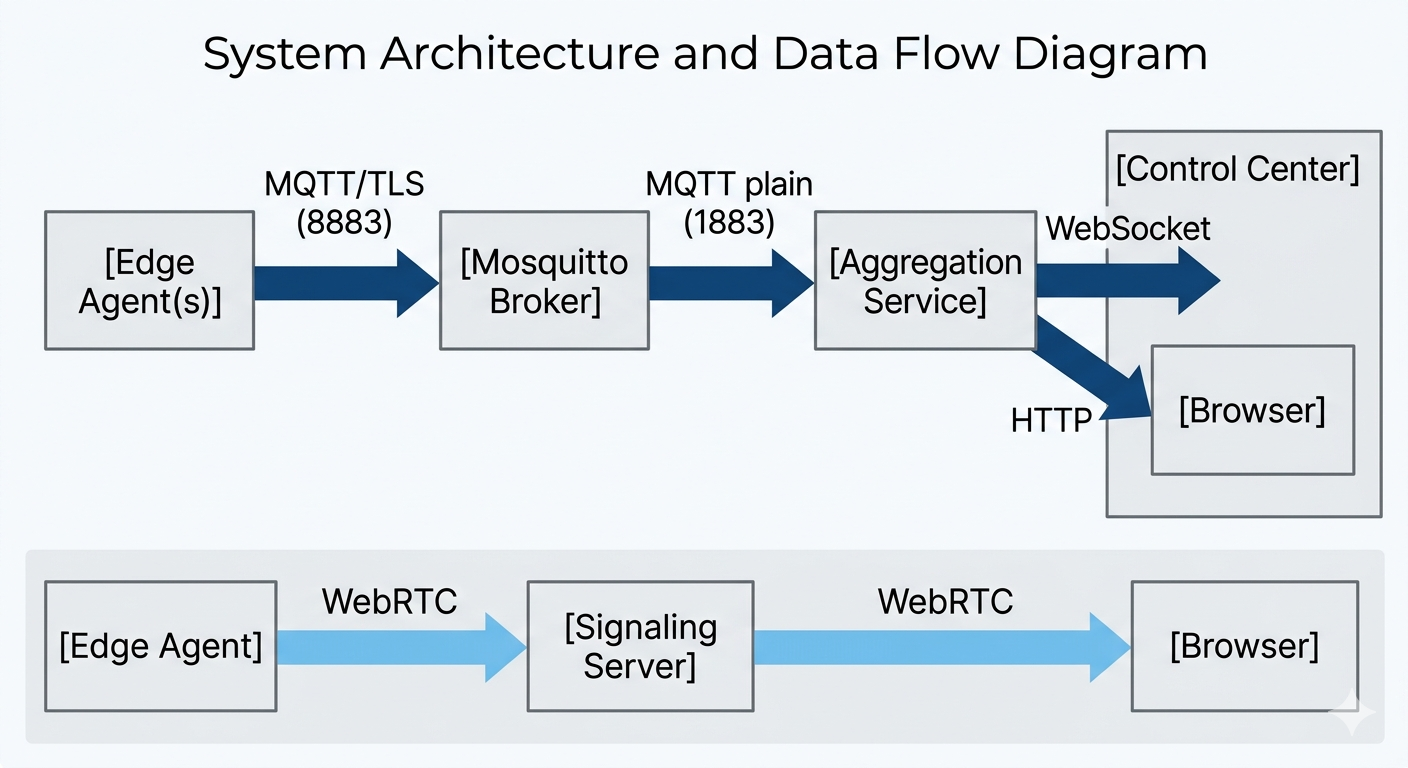
\includegraphics[width=\textwidth]{system_arch.png}
\caption{High-level distributed system architecture}
\label{fig:arch}
\end{figure}

\section{Hardware and Network Setup}

The system was implemented and tested on two commodity laptops running CachyOS
(Arch Linux), connected via a shared WiFi hotspot. An Android smartphone running
the IP Webcam application provided an MJPEG video stream over HTTP. The network
topology assigns addresses in the \texttt{192.168.x.x/24} subnet, with the main
device hosting the Docker stack and the edge device running the Python inference
pipeline.

\section{Model Training Experiments}

Two training experiments were conducted to evaluate different model architectures
and task formulations for UAV detection.

\subsection{Experiment 1: YOLOv12 Medium — Single-Class Drone Detection}

\subsubsection{Configuration}

The first experiment trained a YOLOv12 Medium model on a single-class drone
detection dataset. Training was conducted for 100 epochs with a batch size of 8
at 640$\times$640 resolution using the SGD optimizer with cosine annealing
learning rate schedule.

\begin{table}[H]
\centering
\caption{Experiment 1 Training Configuration}
\begin{tabular}{@{}ll@{}}
\toprule
\textbf{Parameter} & \textbf{Value} \\
\midrule
Model & YOLOv12 Medium \\
Task & Object Detection (single class: drone) \\
Image size & 640$\times$640 \\
Epochs & 100 \\
Batch size & 8 \\
Optimizer & SGD with cosine annealing \\
Classes & 1 (drone) \\
\bottomrule
\end{tabular}
\end{table}

\subsubsection{Results}

\begin{table}[H]
\centering
\caption{Experiment 1 — Best Validation Metrics (Epoch 73)}
\begin{tabular}{@{}ll@{}}
\toprule
\textbf{Metric} & \textbf{Value} \\
\midrule
mAP50 & 0.9159 \\
mAP50-95 & 0.4926 \\
Precision & 0.9879 \\
Recall & 0.7778 \\
Final train box loss & 0.8591 \\
Final val box loss & 1.7353 \\
Total training time & $\sim$44 minutes \\
\bottomrule
\end{tabular}
\end{table}

The model achieved a peak mAP50 of \textbf{91.59\%} at epoch 73, with near-perfect
precision of 98.79\%. The recall of 77.78\% indicates that while the model is
highly confident in its positive detections, it misses approximately one in five
drone instances — likely small or partially occluded targets. The gap between
mAP50 (0.916) and mAP50-95 (0.493) suggests that while the model correctly
identifies drone locations at a relaxed IoU threshold, tighter localization
accuracy requires further improvement.

\begin{figure}[H]
\centering
\begin{subfigure}[b]{0.48\textwidth}
  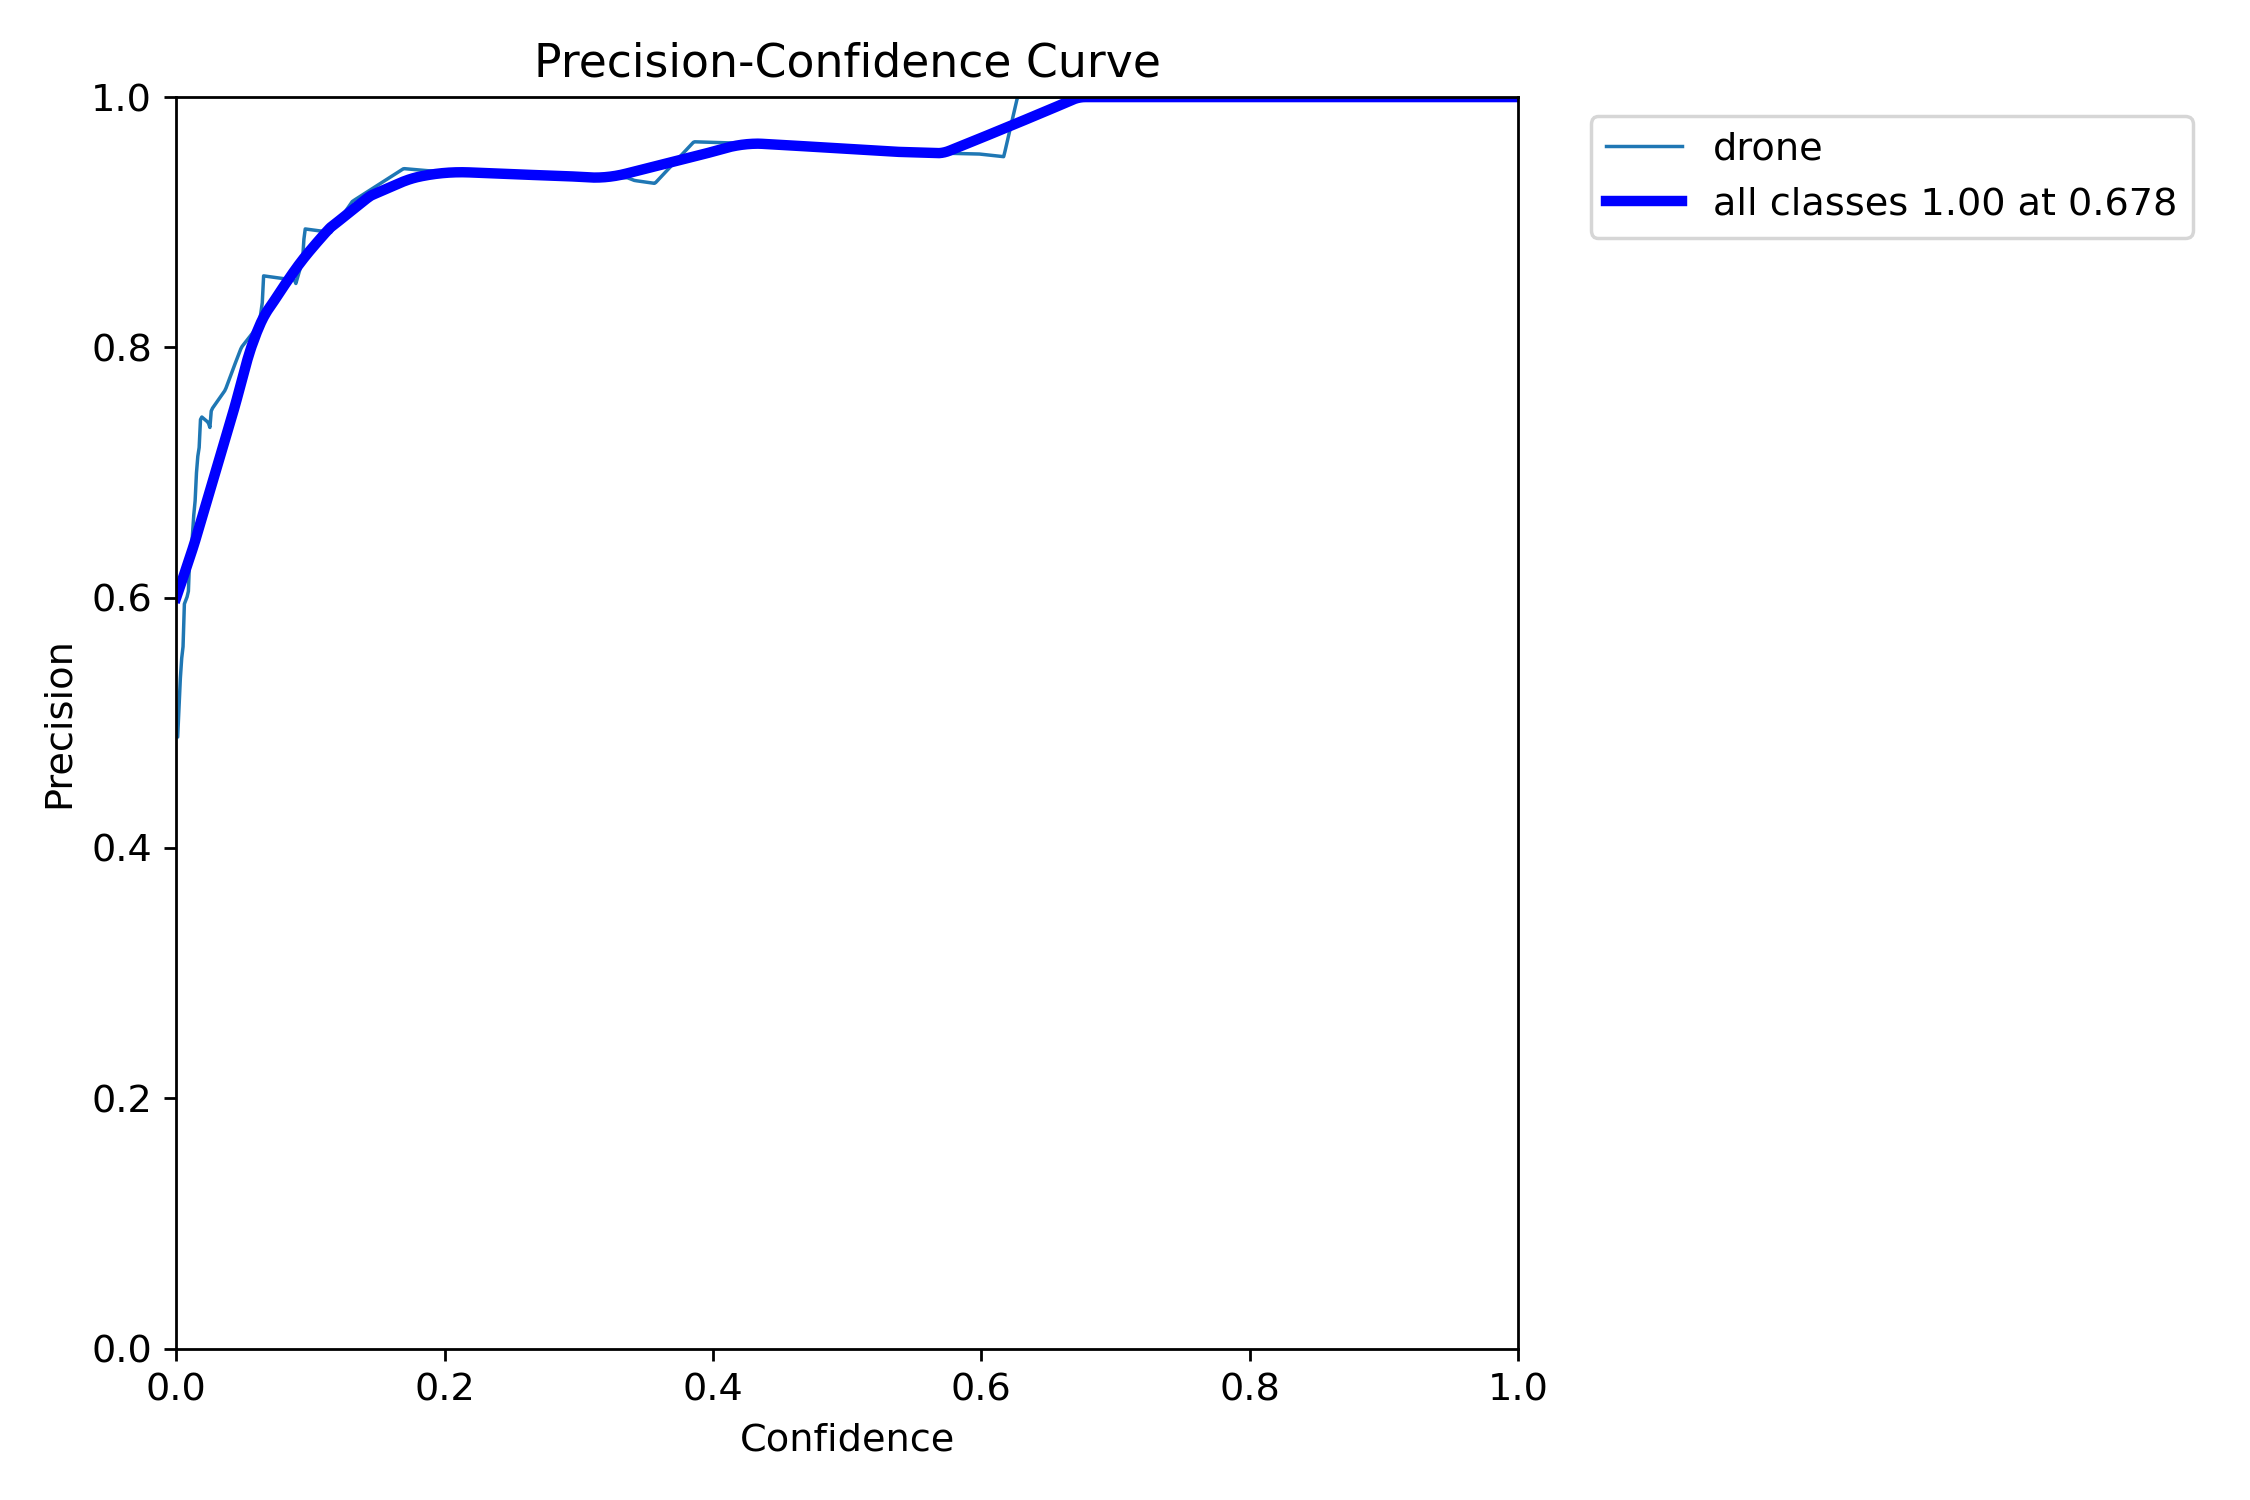
\includegraphics[width=\textwidth]{t1_precision.png}
  \caption{Precision curve}
\end{subfigure}
\hfill
\begin{subfigure}[b]{0.48\textwidth}
  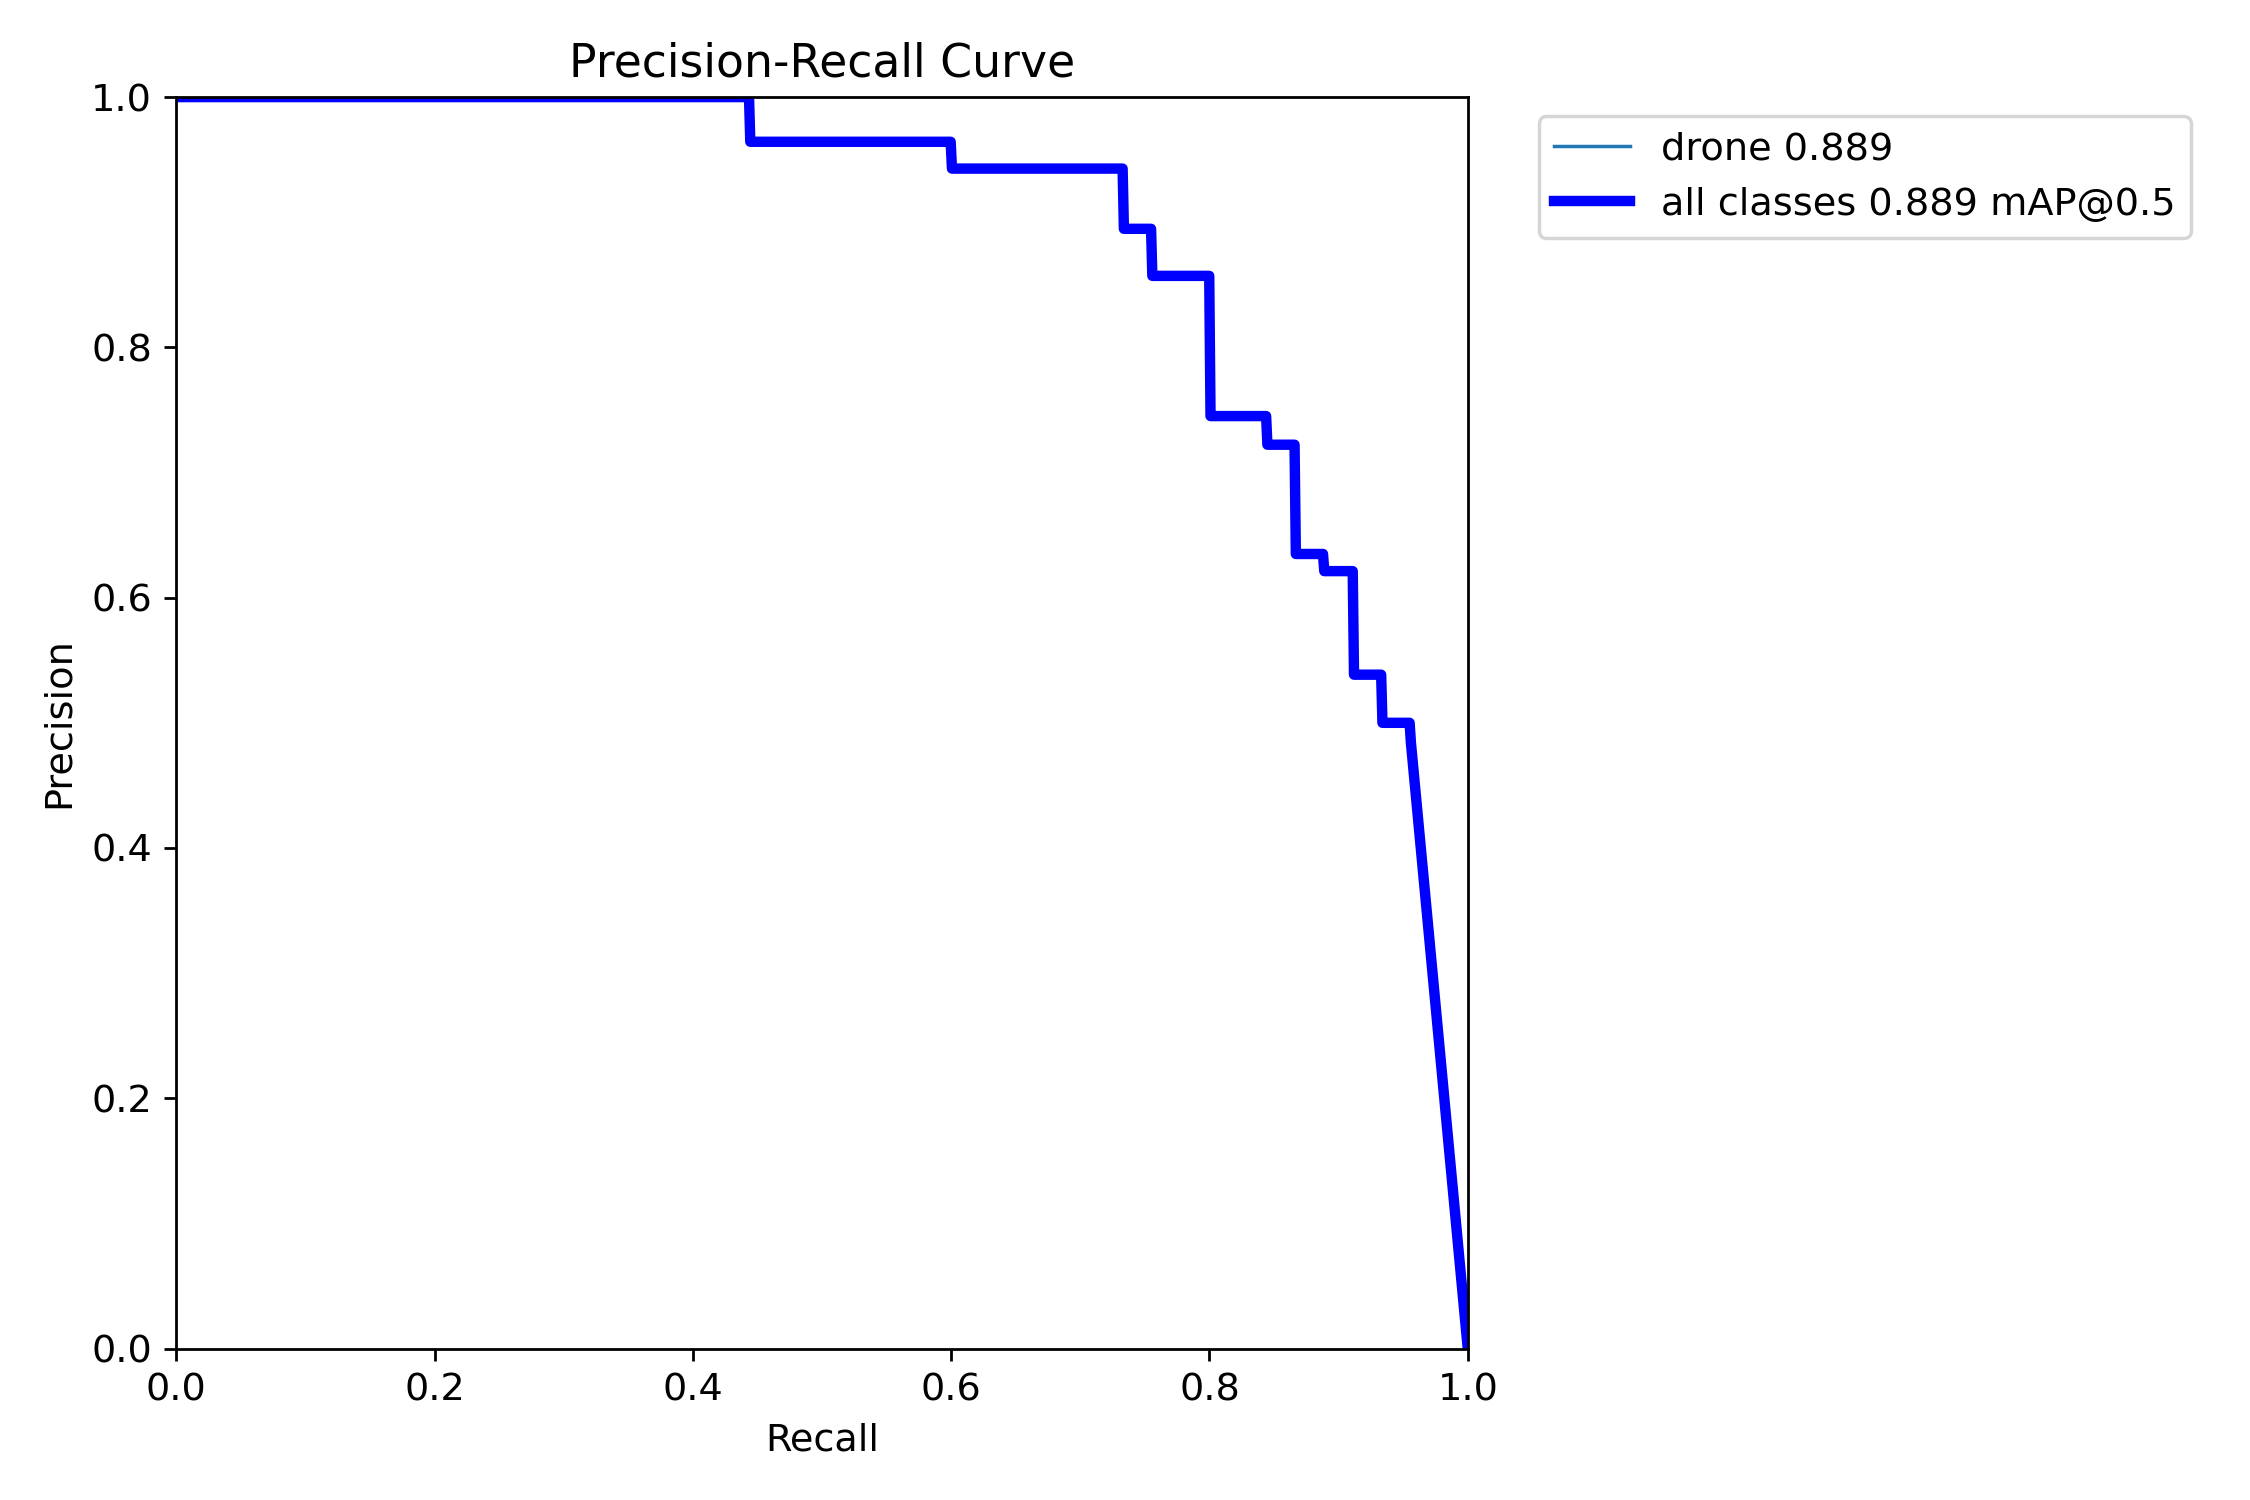
\includegraphics[width=\textwidth]{t1_pr_curve.png}
  \caption{Precision-Recall curve}
\end{subfigure}
\caption{Experiment 1 — YOLOv12 Medium detection performance curves}
\label{fig:test1_curves}
\end{figure}

\begin{figure}[H]
\centering
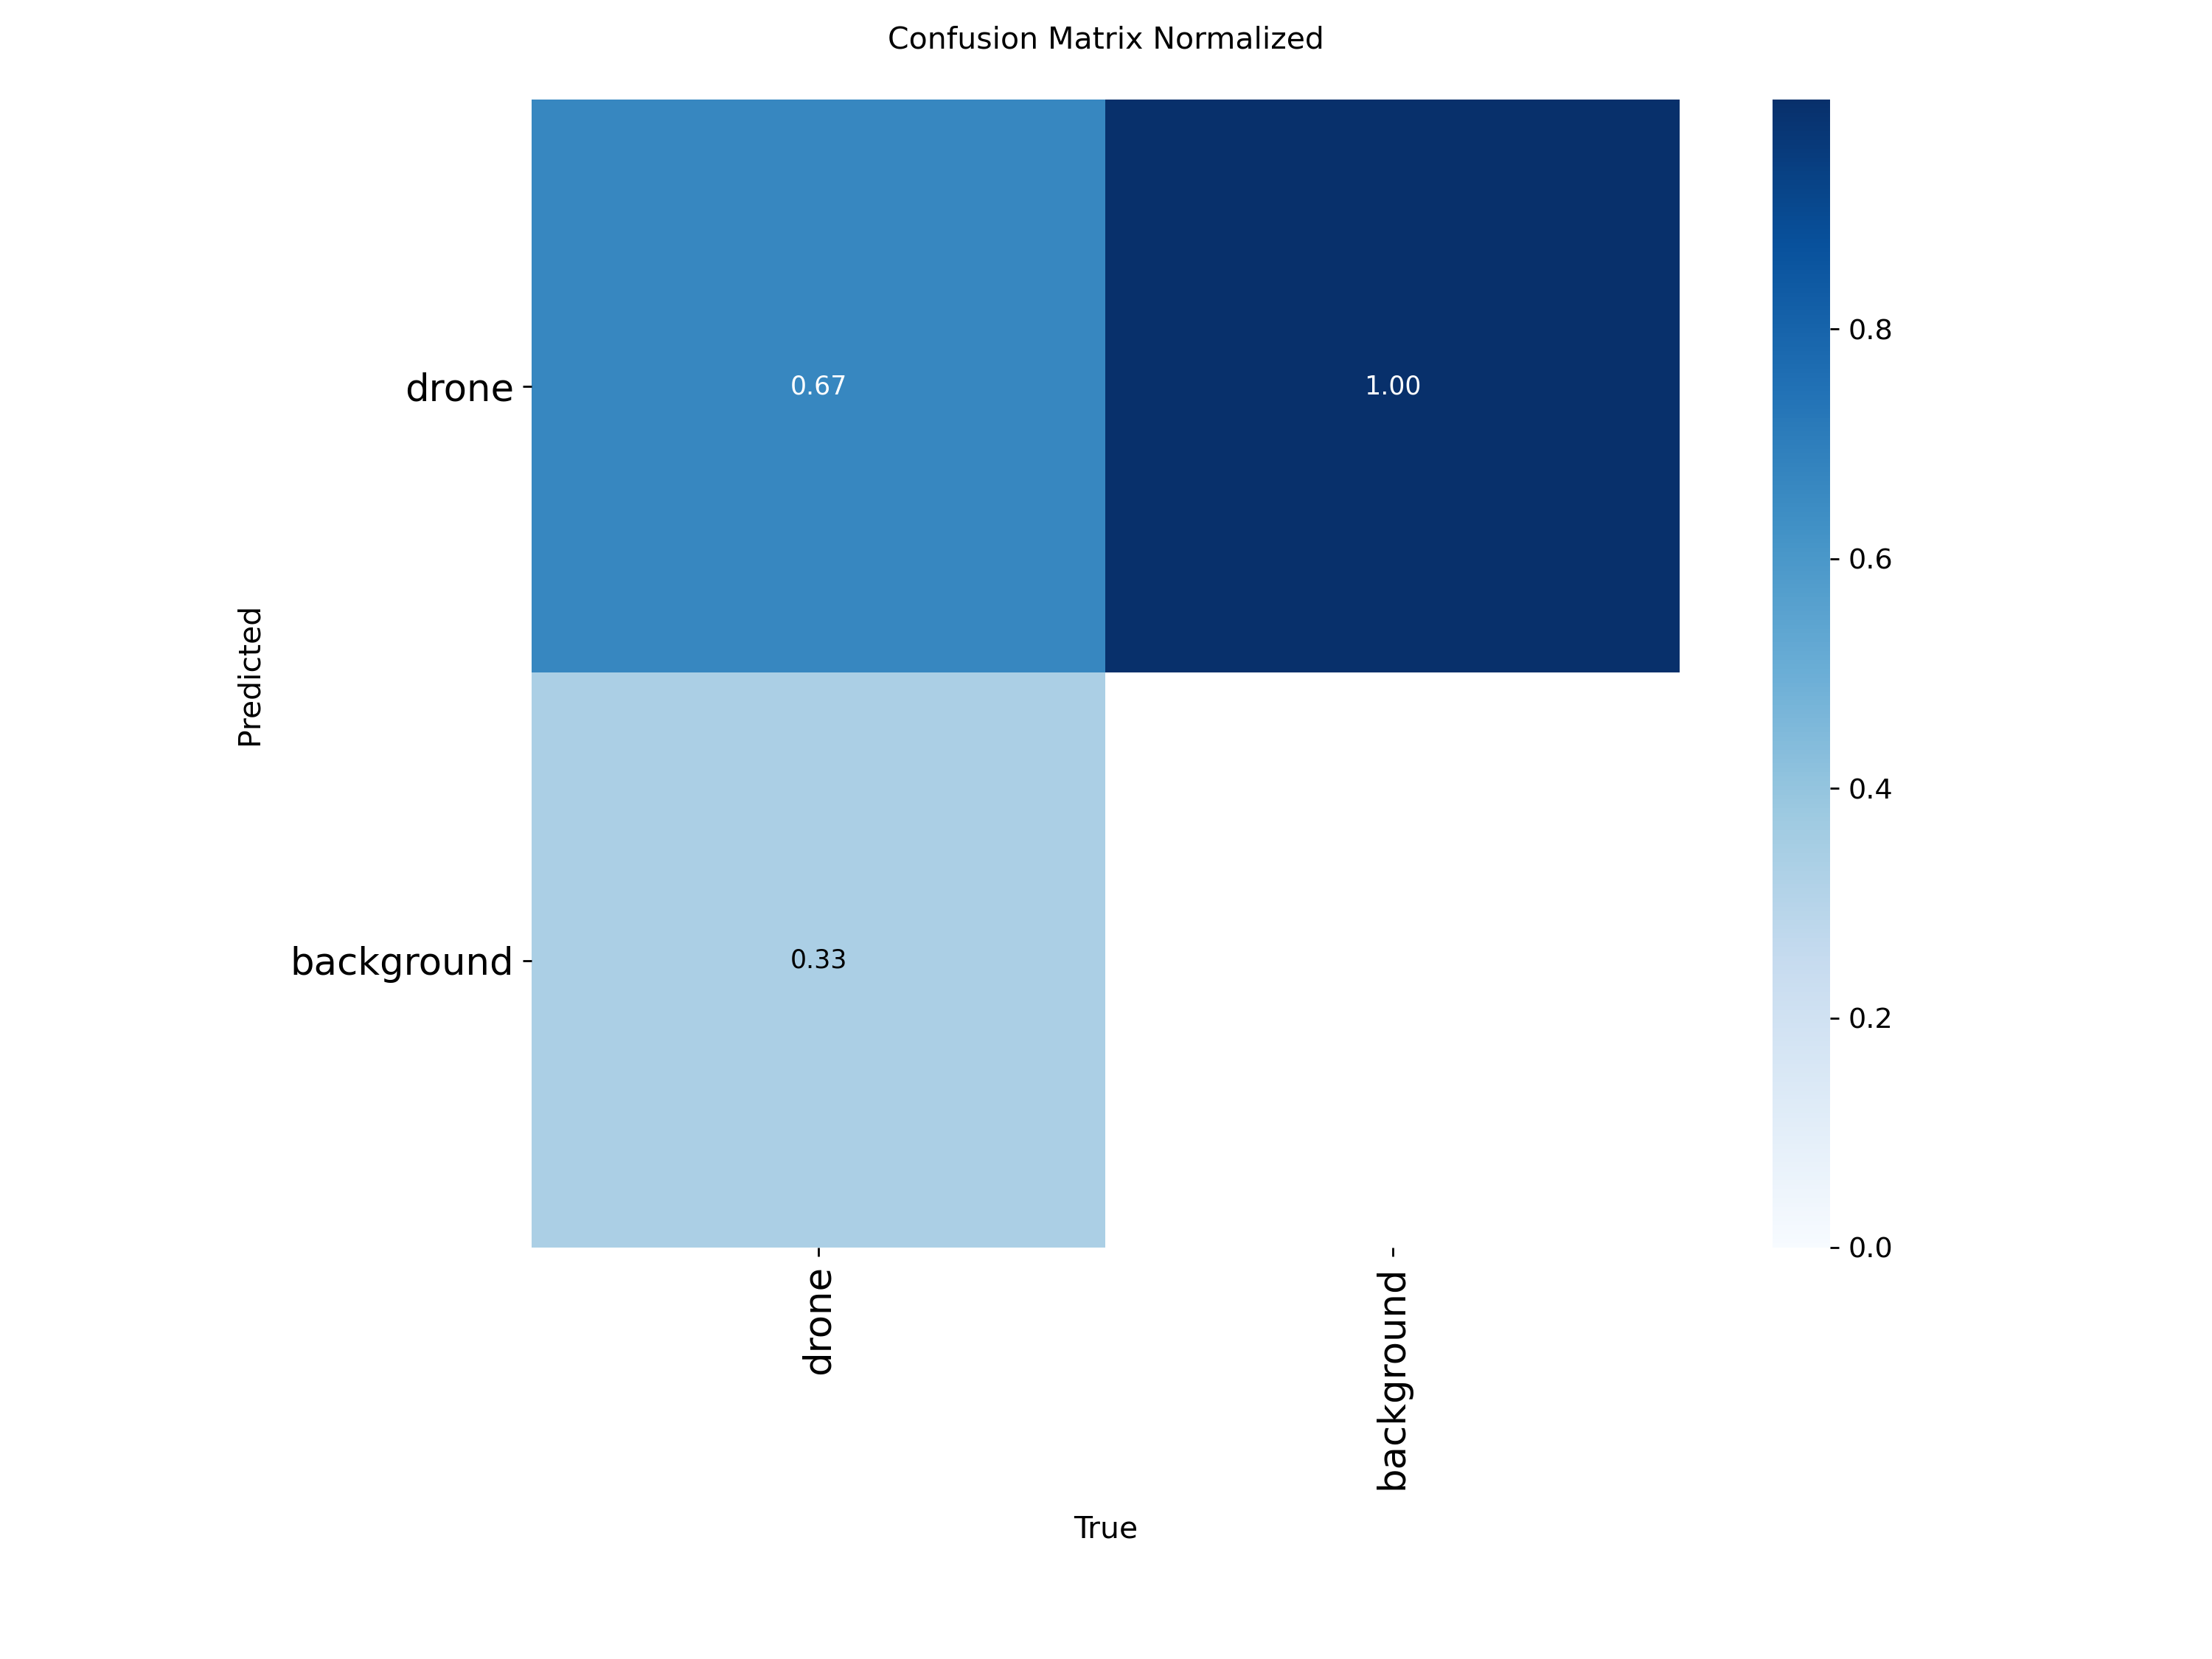
\includegraphics[width=0.6\textwidth]{t1_confusion.png}
\caption{Experiment 1 — Normalized confusion matrix}
\label{fig:test1_confusion}
\end{figure}

\subsection{Experiment 2: YOLO26 Small — Drone vs. Bird Classification}

\subsubsection{Configuration}

The second experiment trained a YOLO26 Small model on the ``Drone vs Bird v3''
dataset, a two-class detection task requiring the model to distinguish between
drones and birds — a significantly harder problem due to visual similarity between
the two classes. Training was conducted for 160 epochs with a batch size of 16
at 896$\times$896 resolution using the AdamW optimizer with cosine learning rate
scheduling.

\begin{table}[H]
\centering
\caption{Experiment 2 Training Configuration}
\begin{tabular}{@{}ll@{}}
\toprule
\textbf{Parameter} & \textbf{Value} \\
\midrule
Model & YOLO26 Small (yolo26s.pt) \\
Task & Object Detection (2 classes: drone, bird) \\
Dataset & Drone vs Bird v3 (YOLO format) \\
Image size & 896$\times$896 \\
Epochs & 160 \\
Batch size & 16 \\
Optimizer & AdamW \\
Learning rate & 0.002 (cosine decay to 0.01$\times$) \\
Warmup epochs & 5 \\
Augmentation & Mosaic (0.6), MixUp (0.1), RandAugment \\
Hardware & NVIDIA T4 GPU (Google Colab) \\
\bottomrule
\end{tabular}
\end{table}

\subsubsection{Dataset}

The dataset contains labeled images of drones and birds captured under diverse
real-world conditions including varying distances, lighting conditions, backgrounds,
and flight orientations. Figure~\ref{fig:labels} shows the class distribution and
bounding box statistics of the training set.

\begin{figure}[H]
\centering
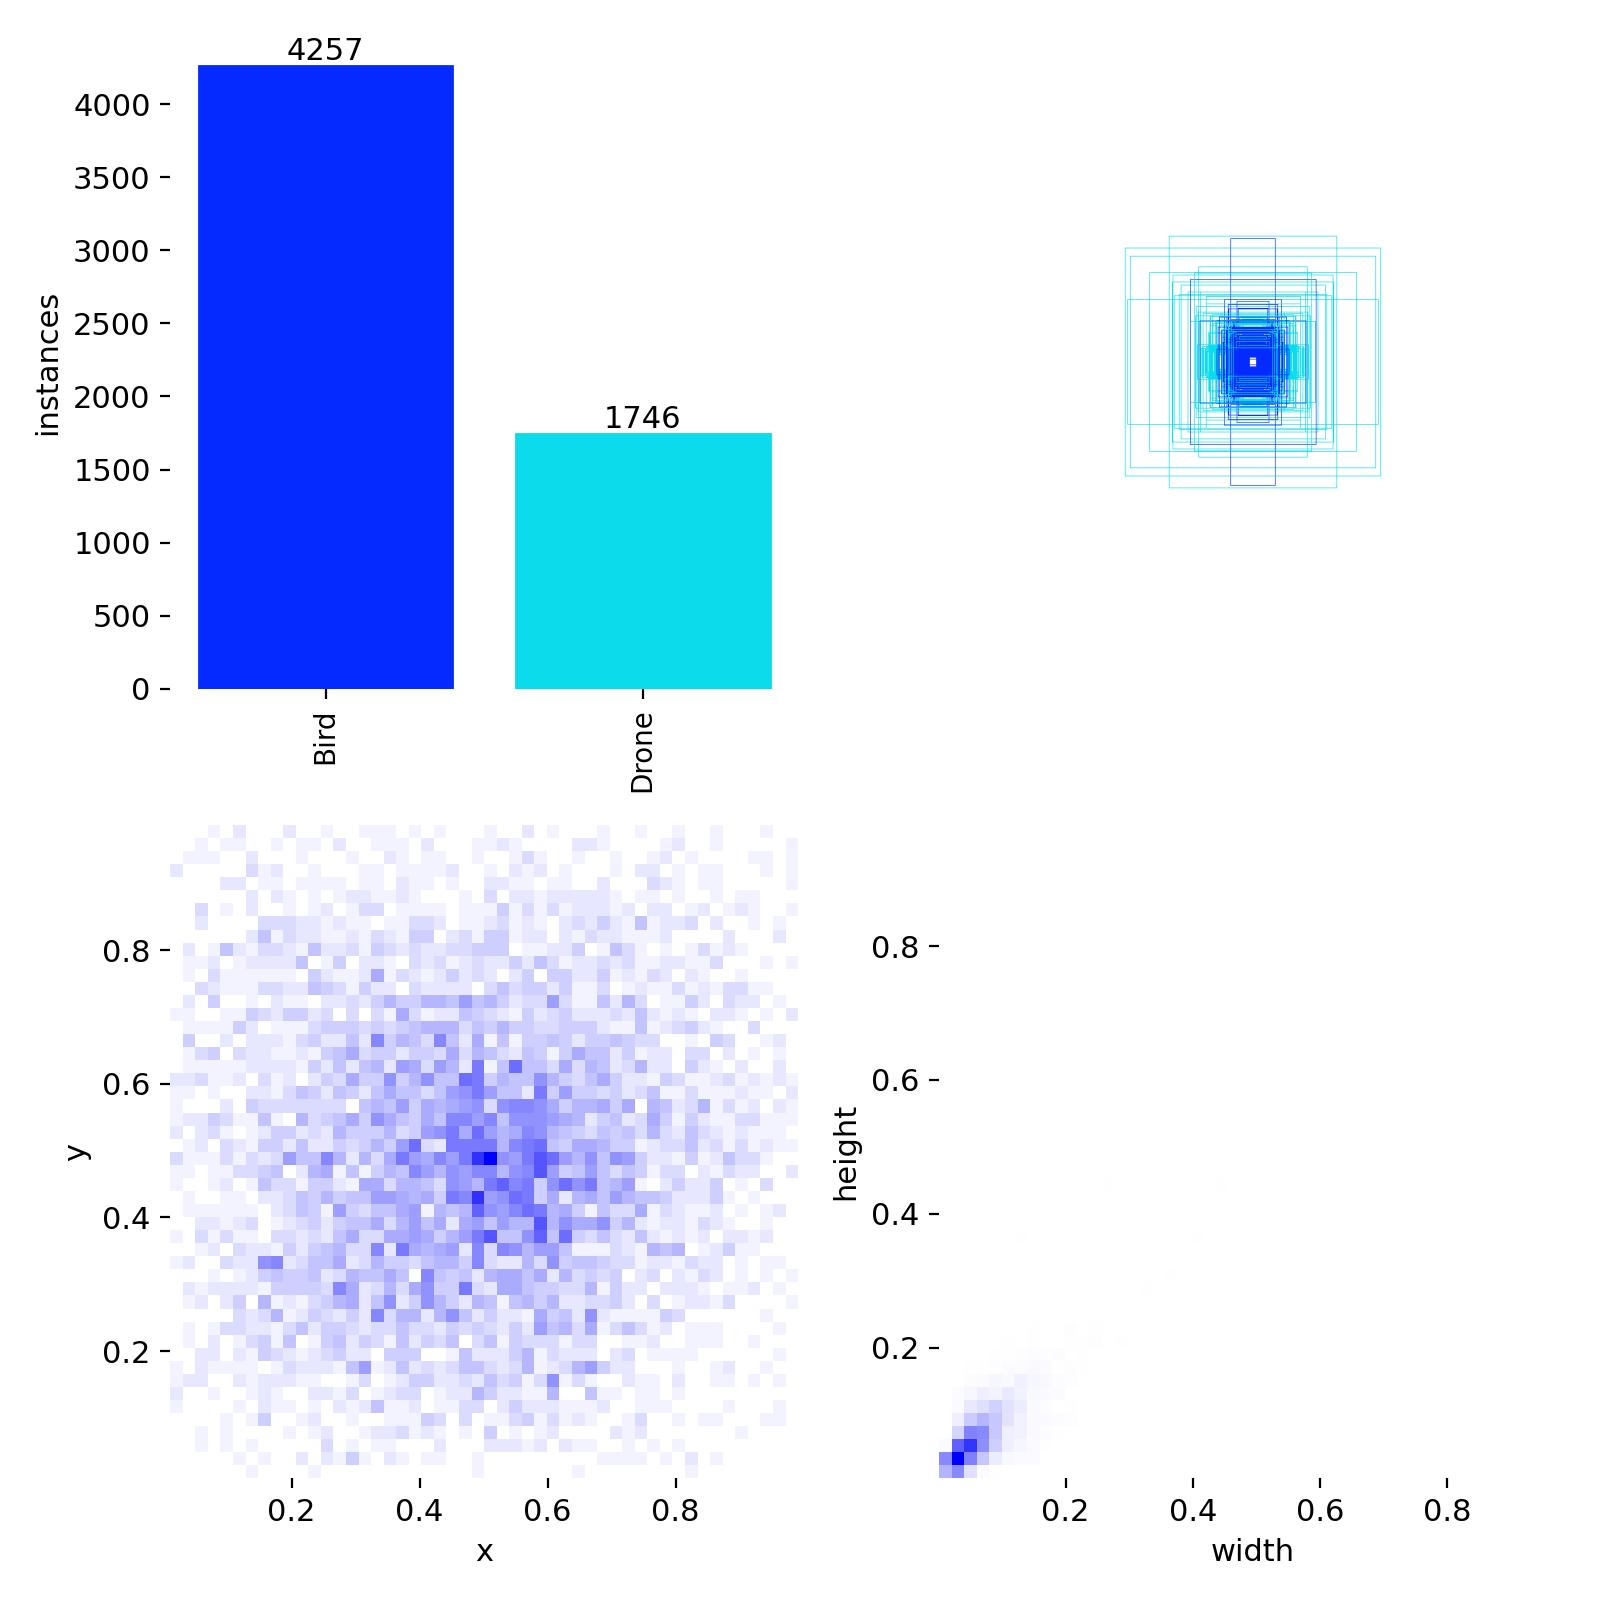
\includegraphics[width=0.7\textwidth]{t2_labels.jpg}
\caption{Experiment 2 — Dataset label distribution and bounding box statistics}
\label{fig:labels}
\end{figure}

\subsubsection{Results}

\begin{table}[H]
\centering
\caption{Experiment 2 — Best Validation Metrics (Epoch 145)}
\begin{tabular}{@{}ll@{}}
\toprule
\textbf{Metric} & \textbf{Value} \\
\midrule
mAP50 & 0.8547 \\
mAP50-95 & 0.4260 \\
Precision & 0.8341 \\
Recall & 0.8093 \\
Final train box loss & 1.5193 \\
Final val box loss & 1.8039 \\
Total training time & $\sim$3.91 hours \\
\bottomrule
\end{tabular}
\end{table}

The YOLO26s model achieved a peak mAP50 of \textbf{85.47\%} on the two-class
drone-vs-bird task at epoch 145. Compared to Experiment 1, the more balanced
precision (83.41\%) and recall (80.93\%) indicate that the model generalizes
better across both classes, avoiding the high-precision/low-recall trade-off
observed in the single-class experiment. The training converged smoothly over
160 epochs, with the loss curves showing consistent improvement throughout.

\begin{figure}[H]
\centering
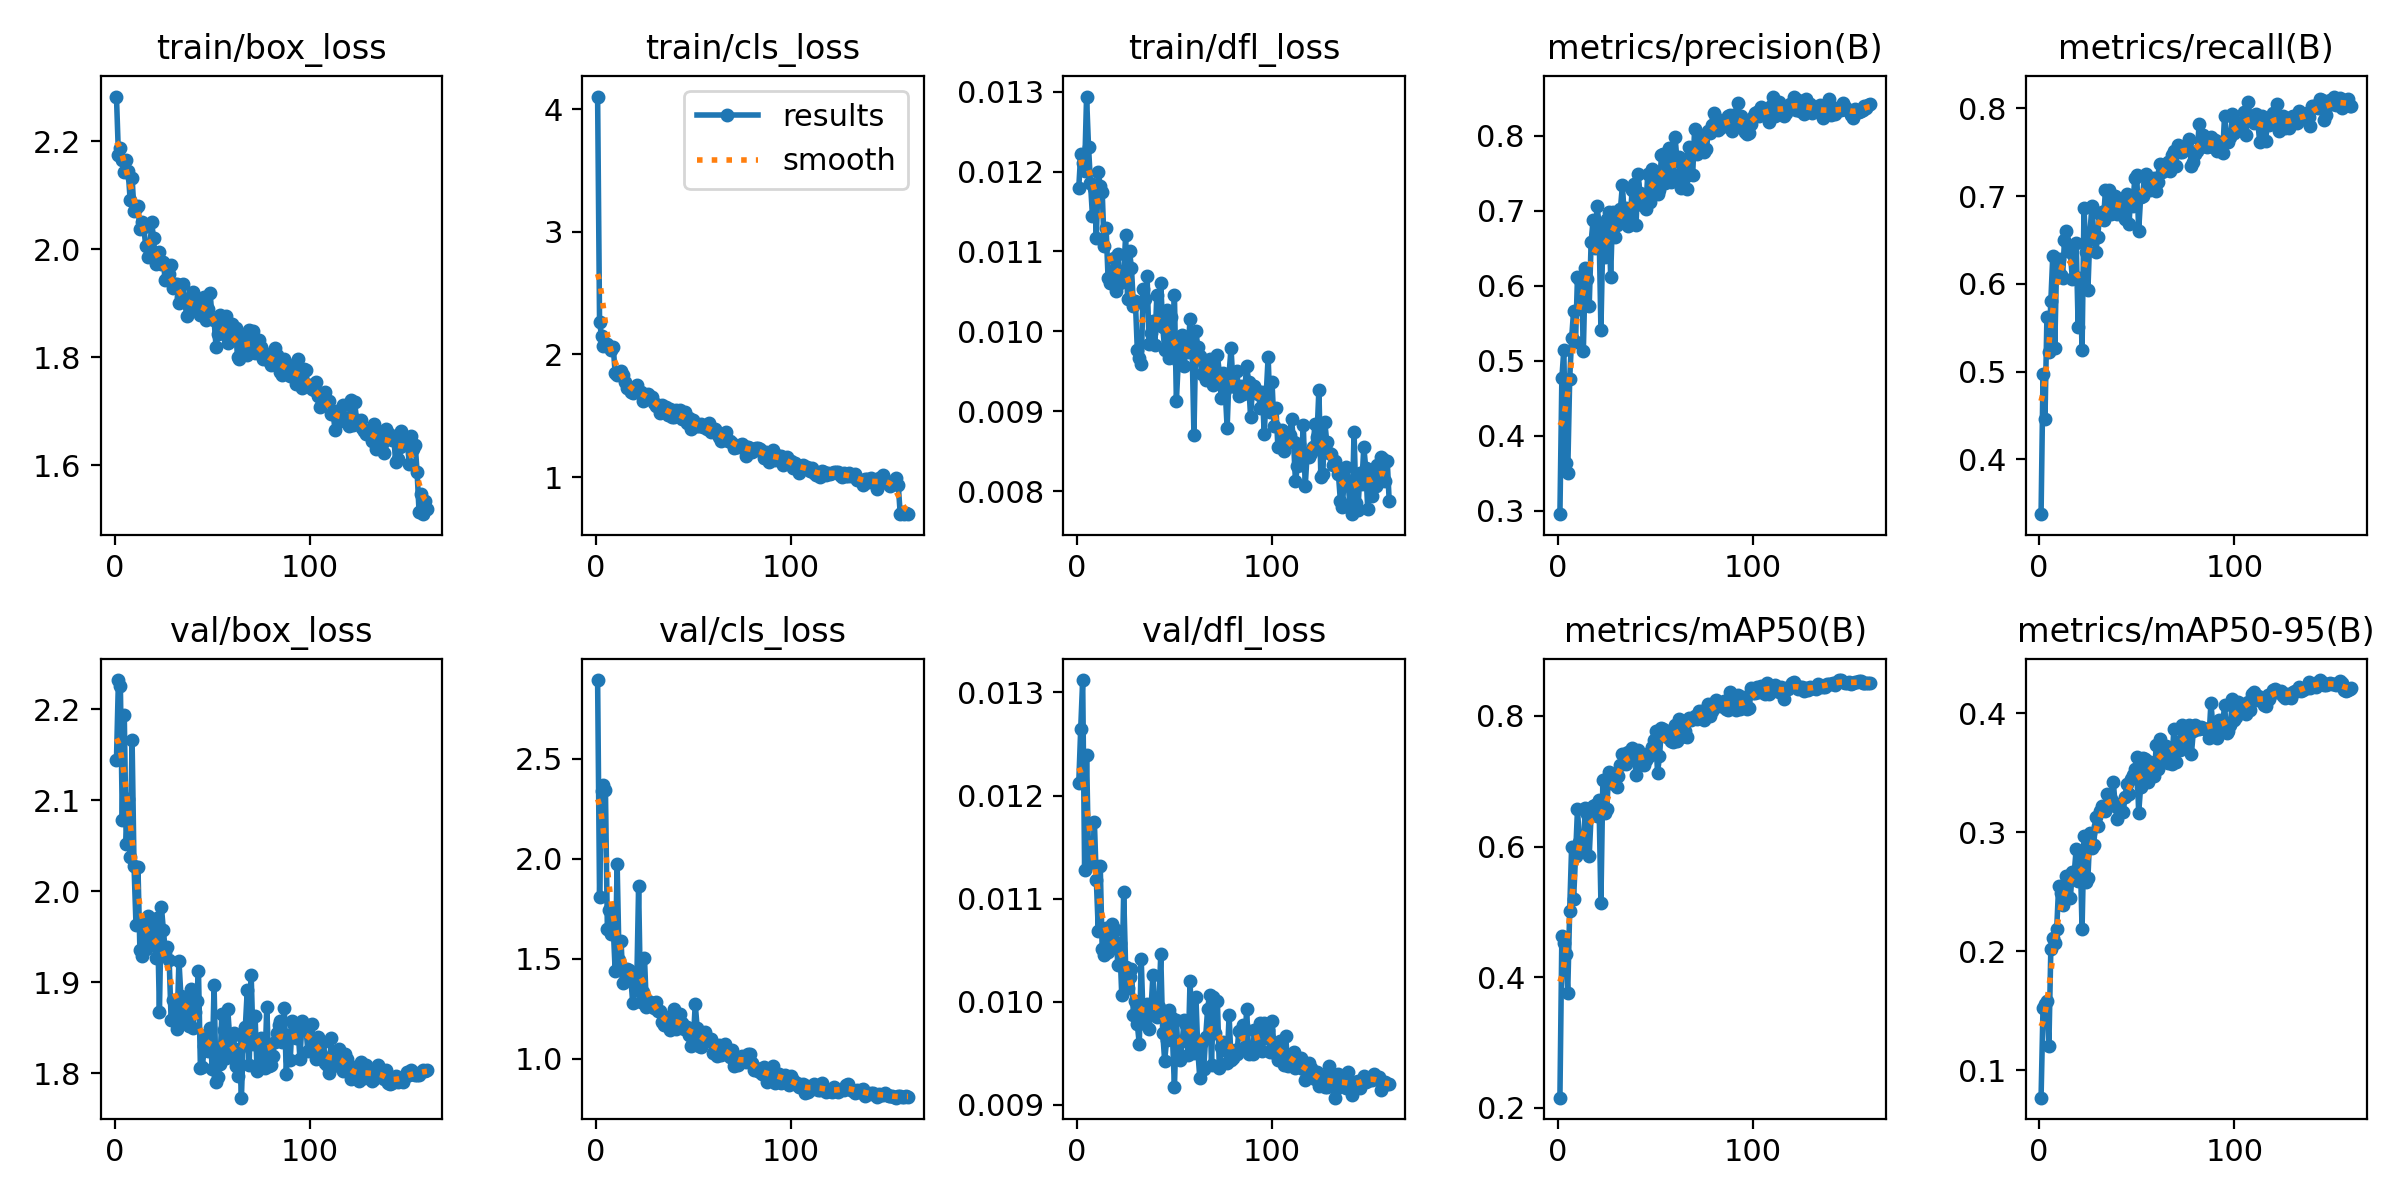
\includegraphics[width=\textwidth]{t2_results.png}
\caption{Experiment 2 — Training and validation metrics over 160 epochs}
\label{fig:test2_results}
\end{figure}

\begin{figure}[H]
\centering
\begin{subfigure}[b]{0.48\textwidth}
  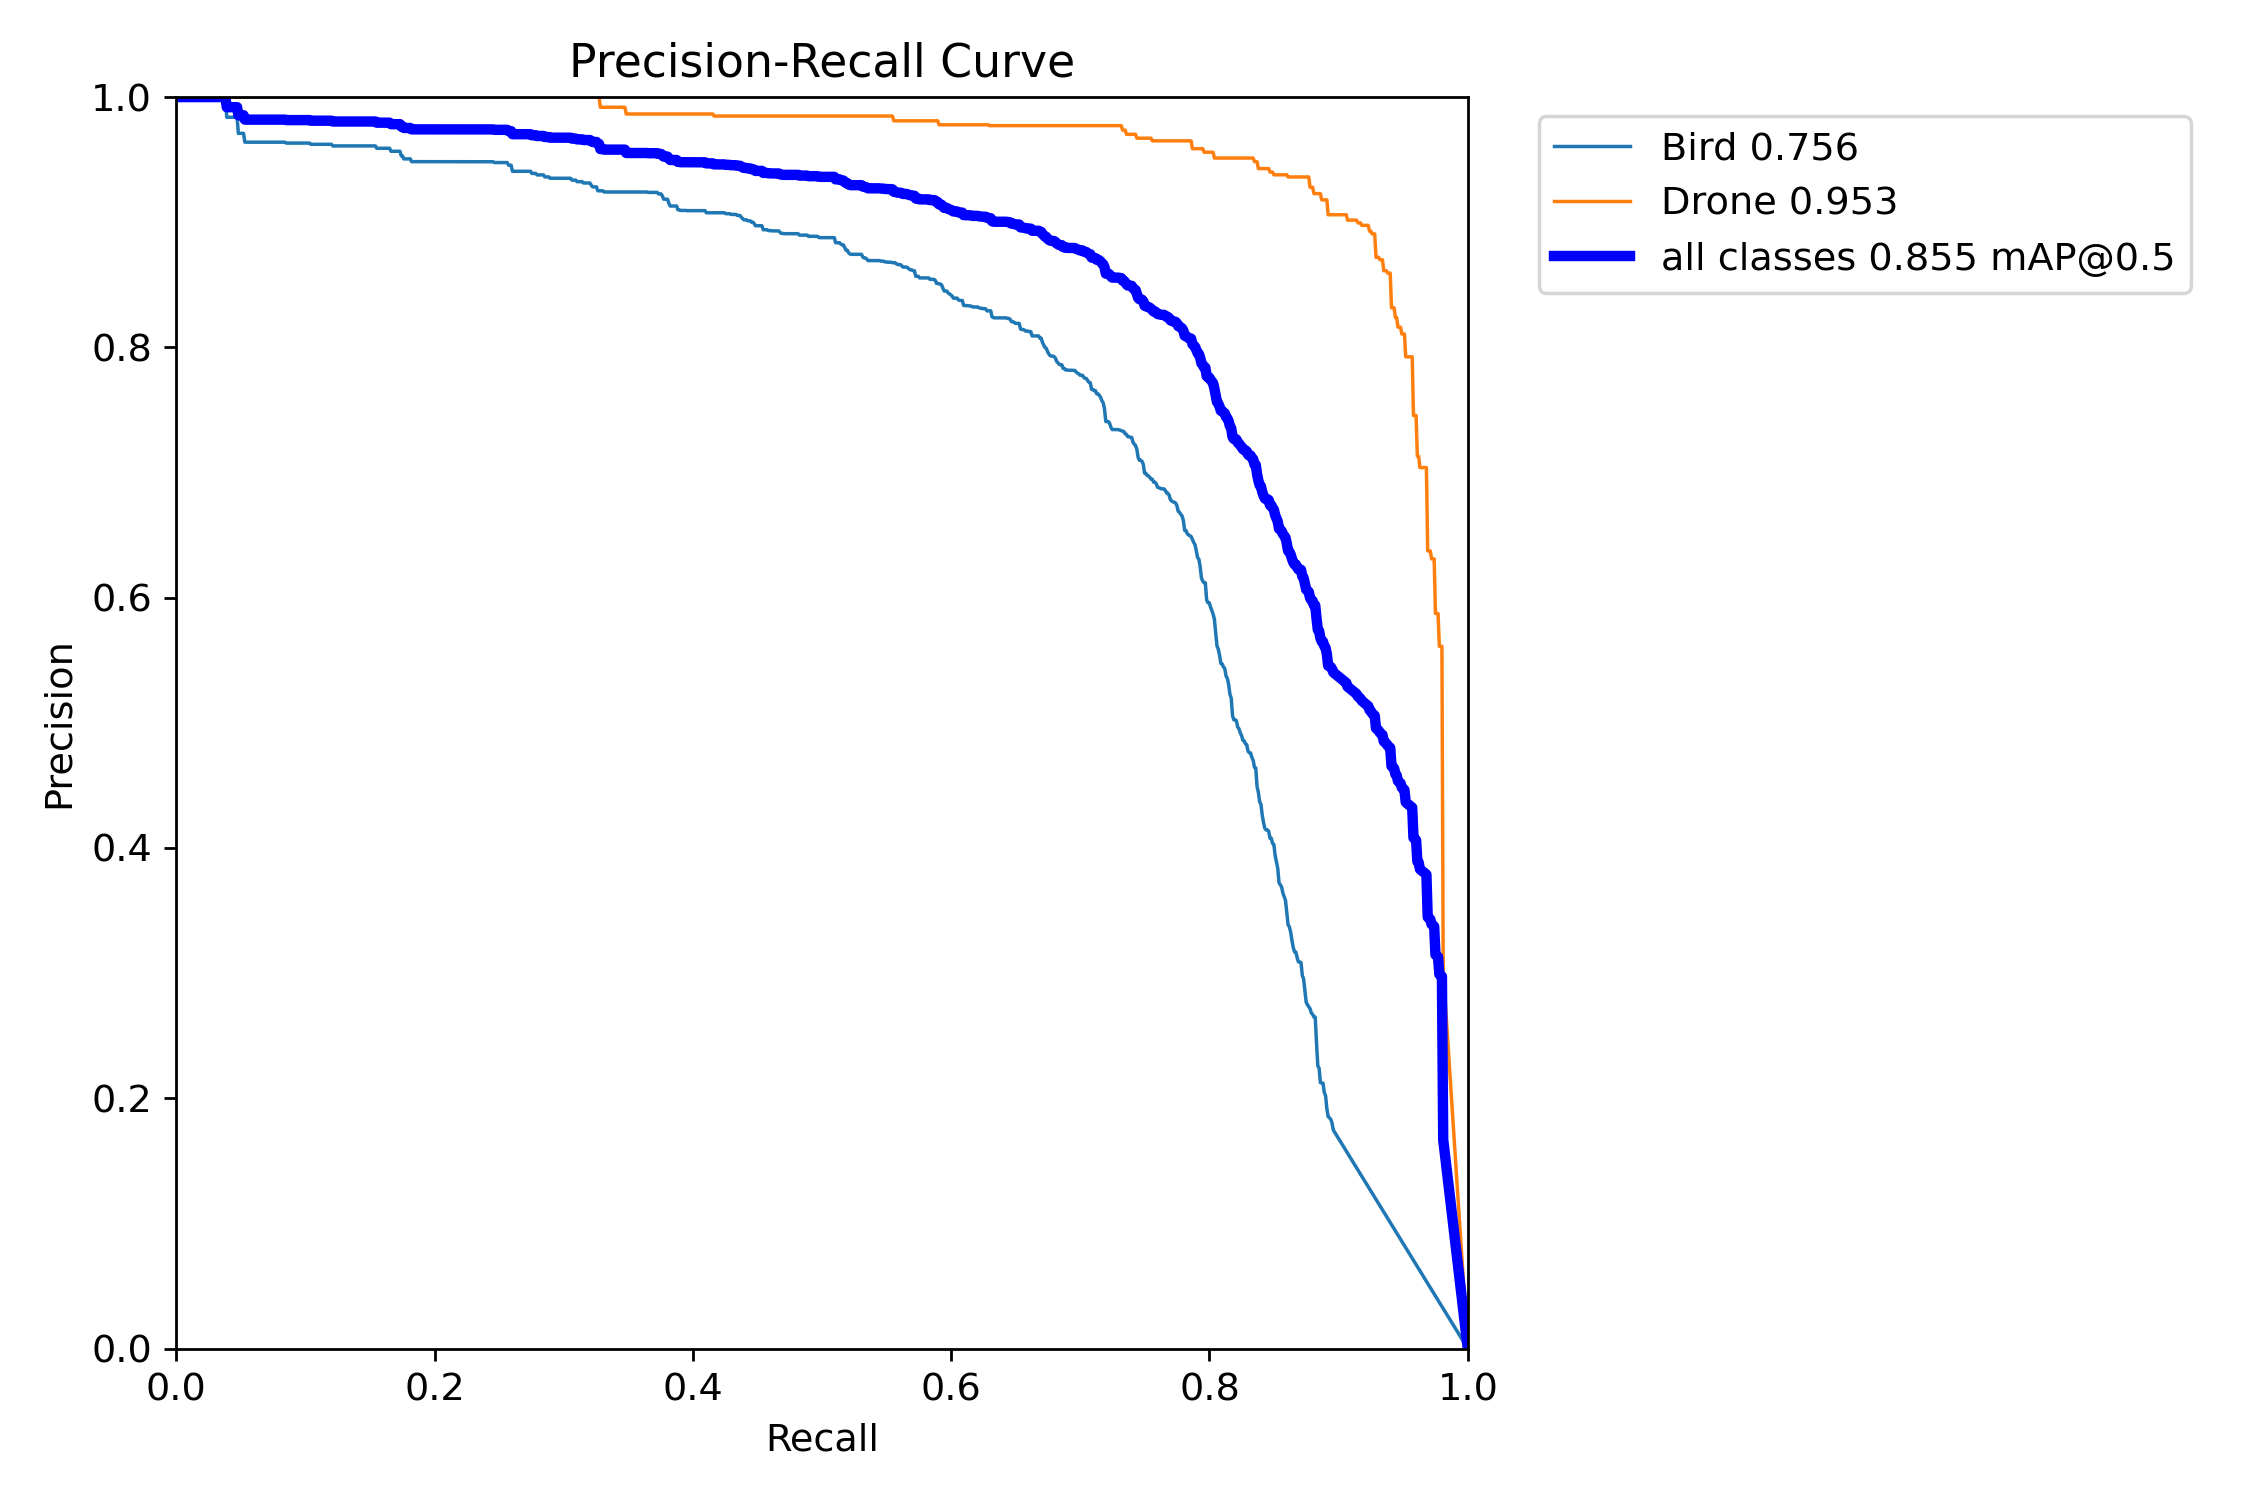
\includegraphics[width=\textwidth]{t2_pr_curve.png}
  \caption{Precision-Recall curve}
\end{subfigure}
\hfill
\begin{subfigure}[b]{0.48\textwidth}
  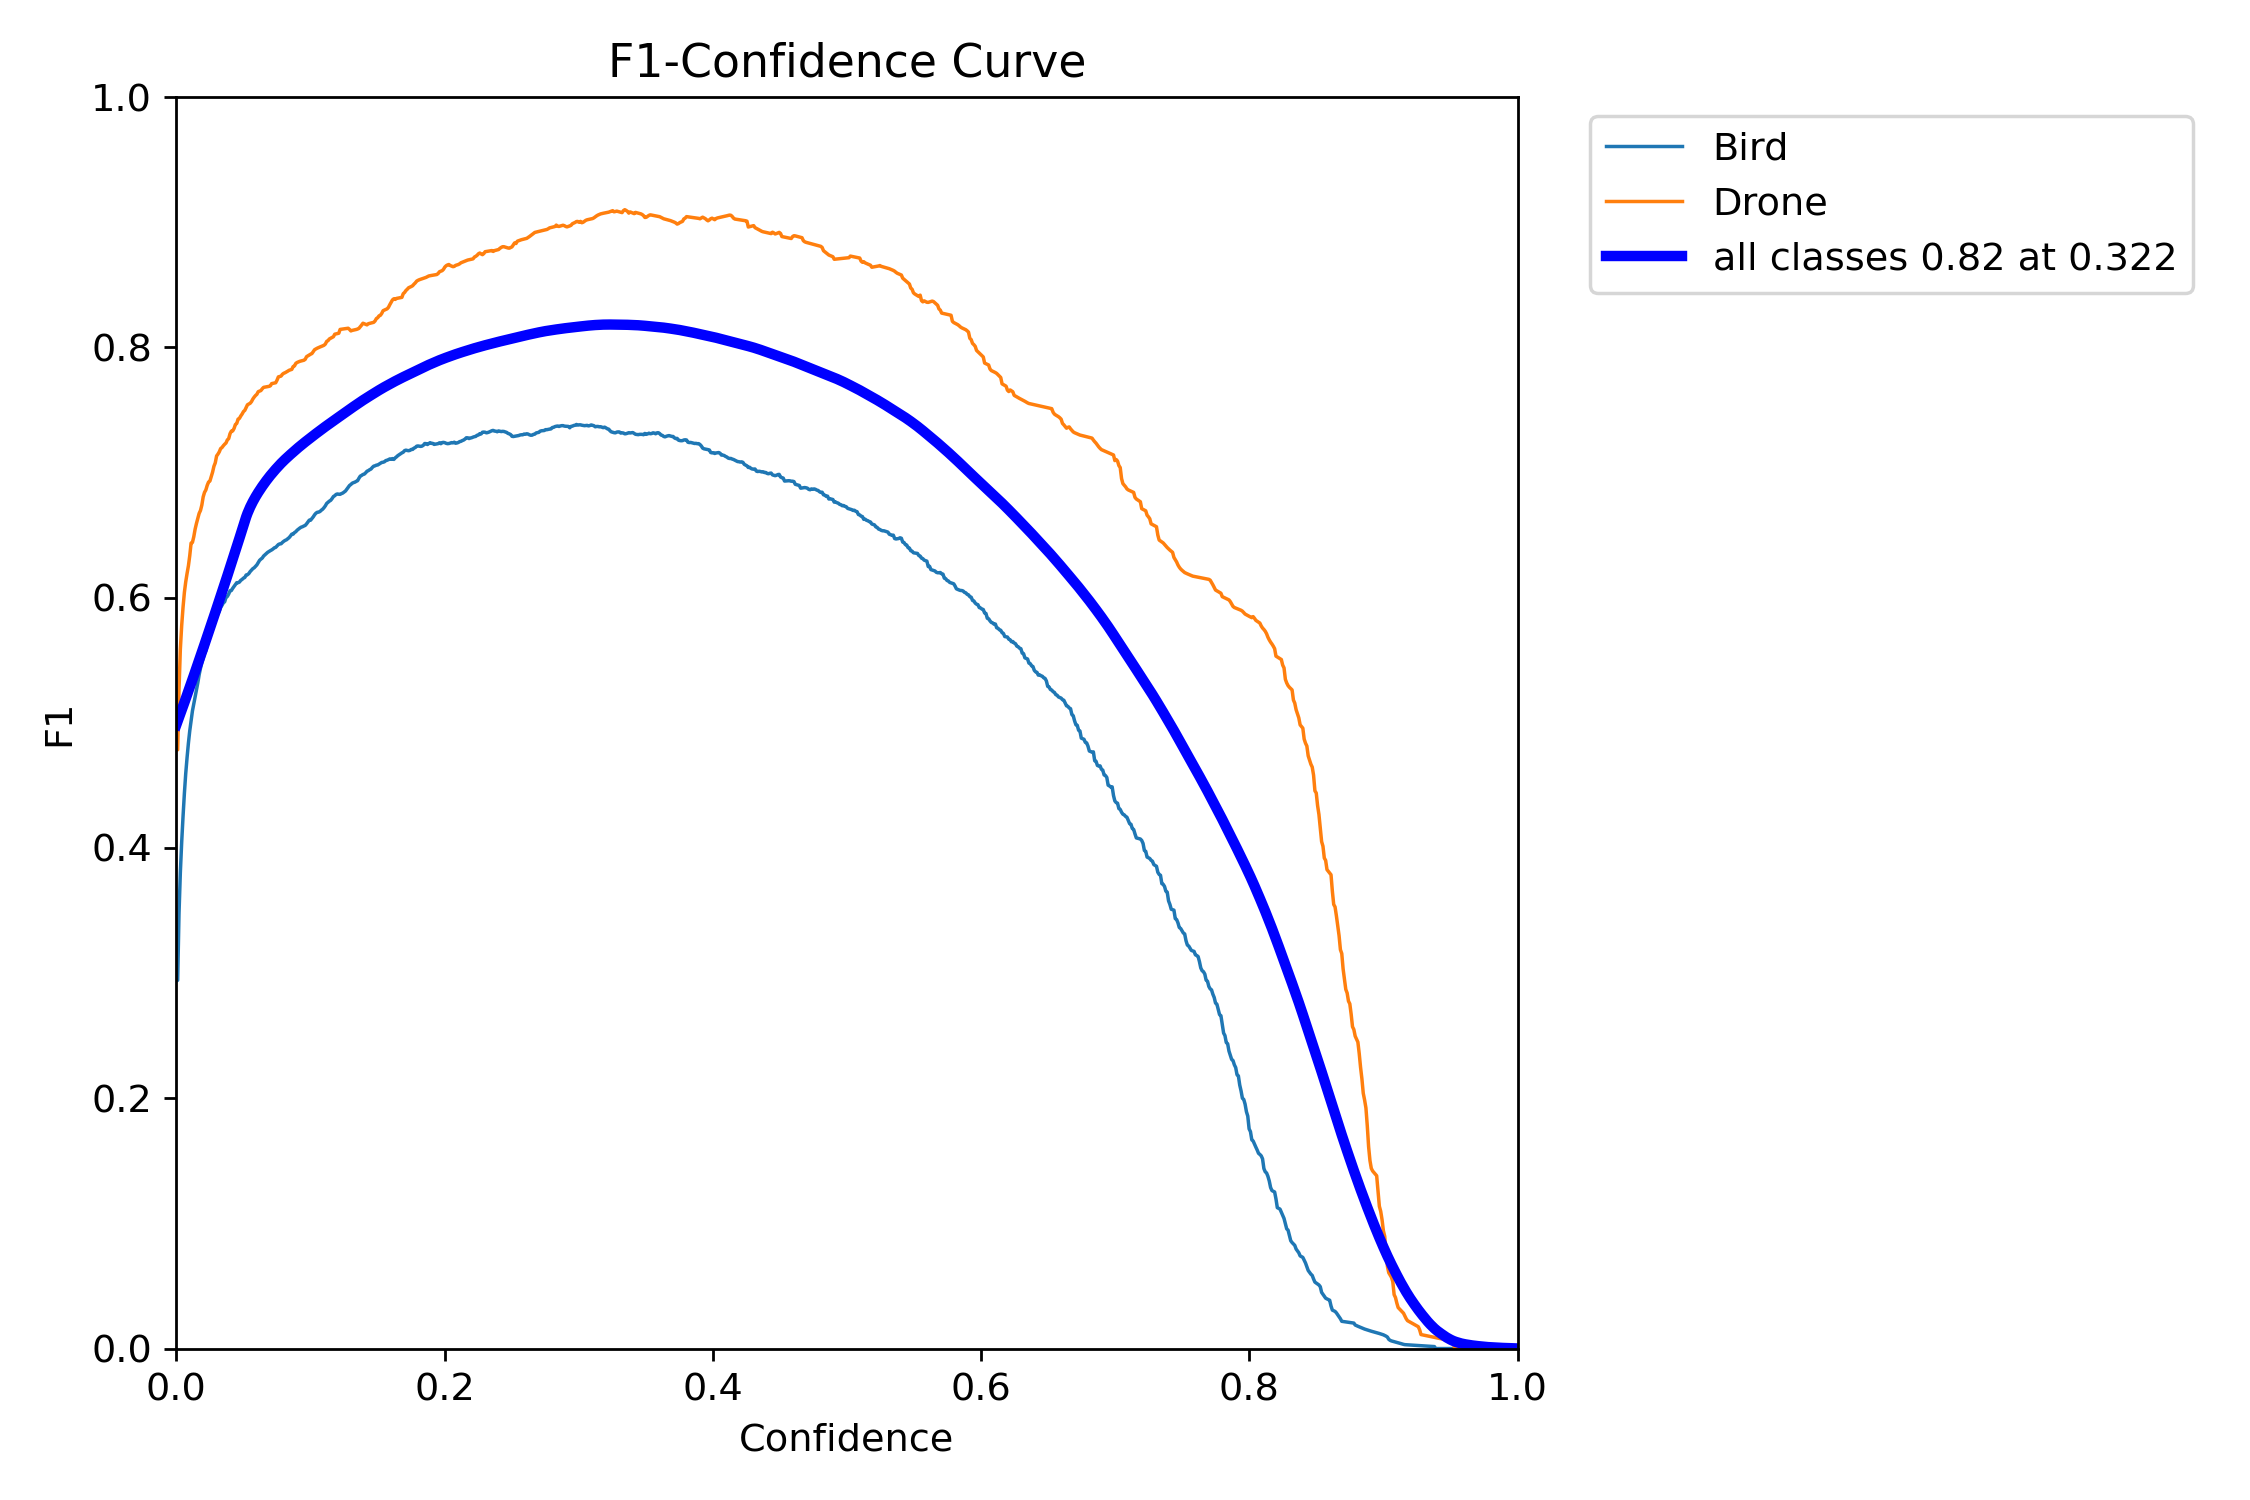
\includegraphics[width=\textwidth]{t2_f1_curve.png}
  \caption{F1-Confidence curve}
\end{subfigure}
\caption{Experiment 2 — YOLO26s detection performance curves}
\label{fig:test2_curves}
\end{figure}

\begin{figure}[H]
\centering
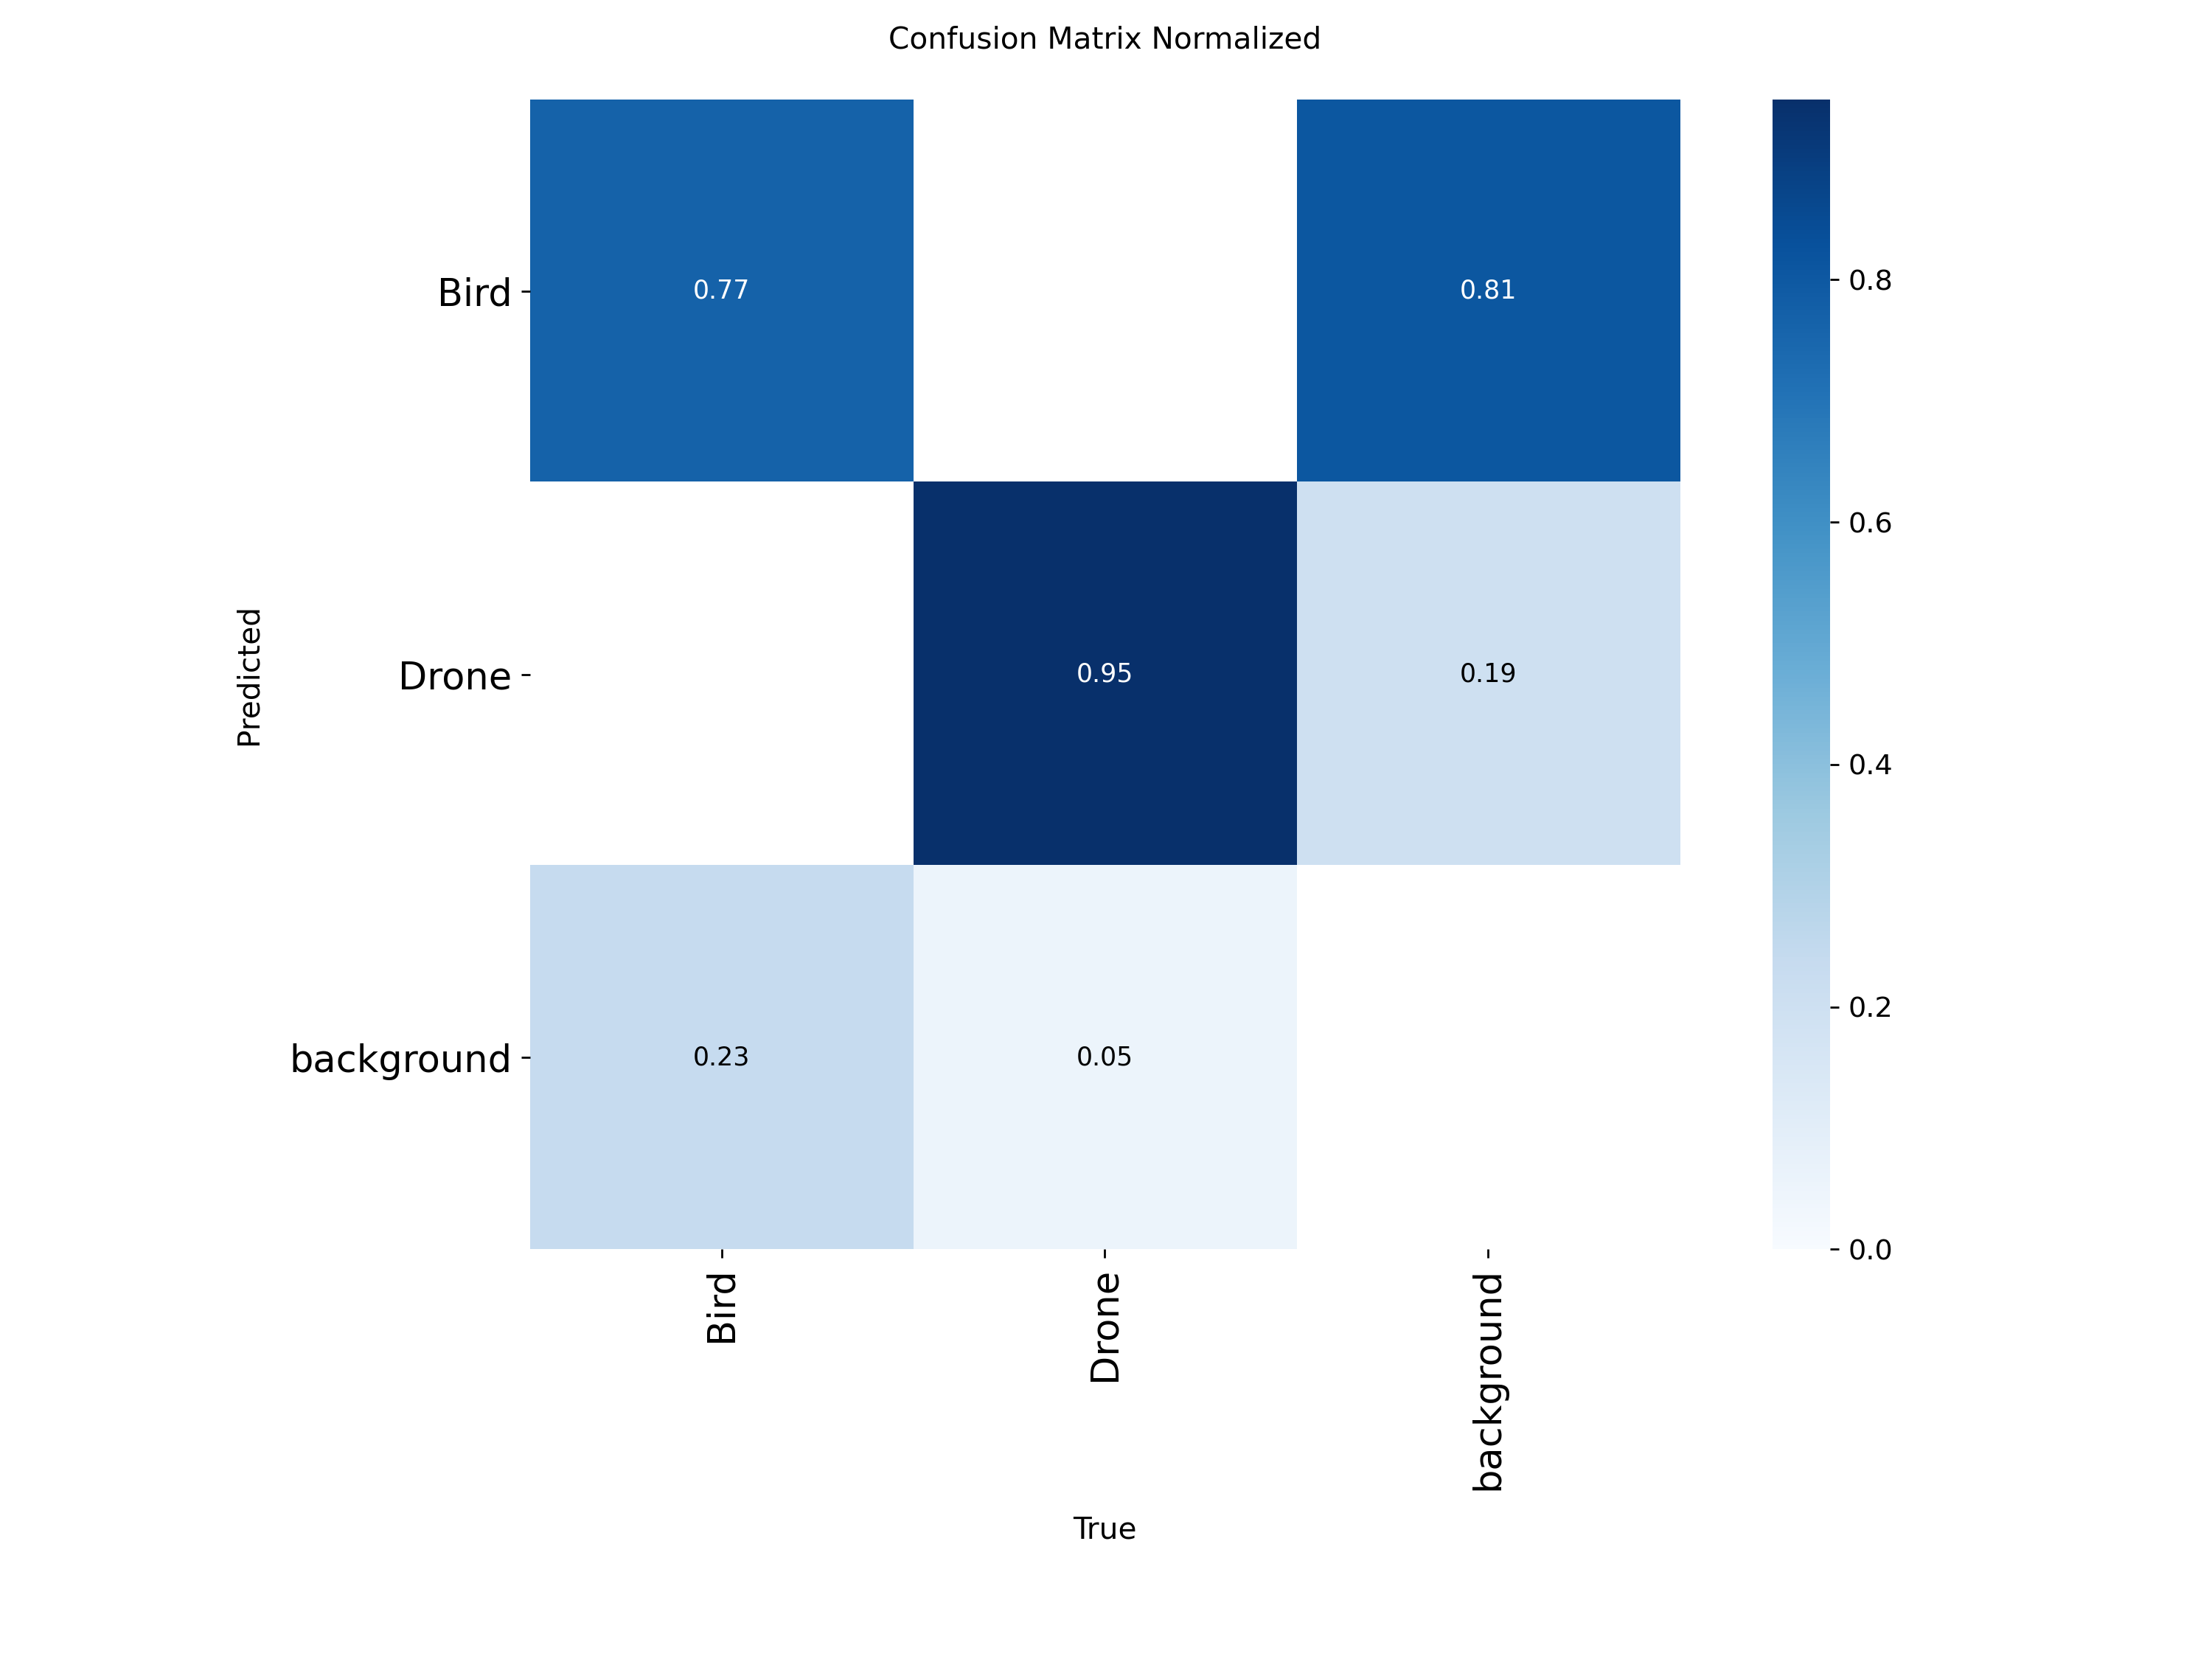
\includegraphics[width=0.6\textwidth]{t2_confusion.png}
\caption{Experiment 2 — Normalized confusion matrix (drone vs. bird)}
\label{fig:test2_confusion}
\end{figure}

\begin{figure}[H]
\centering
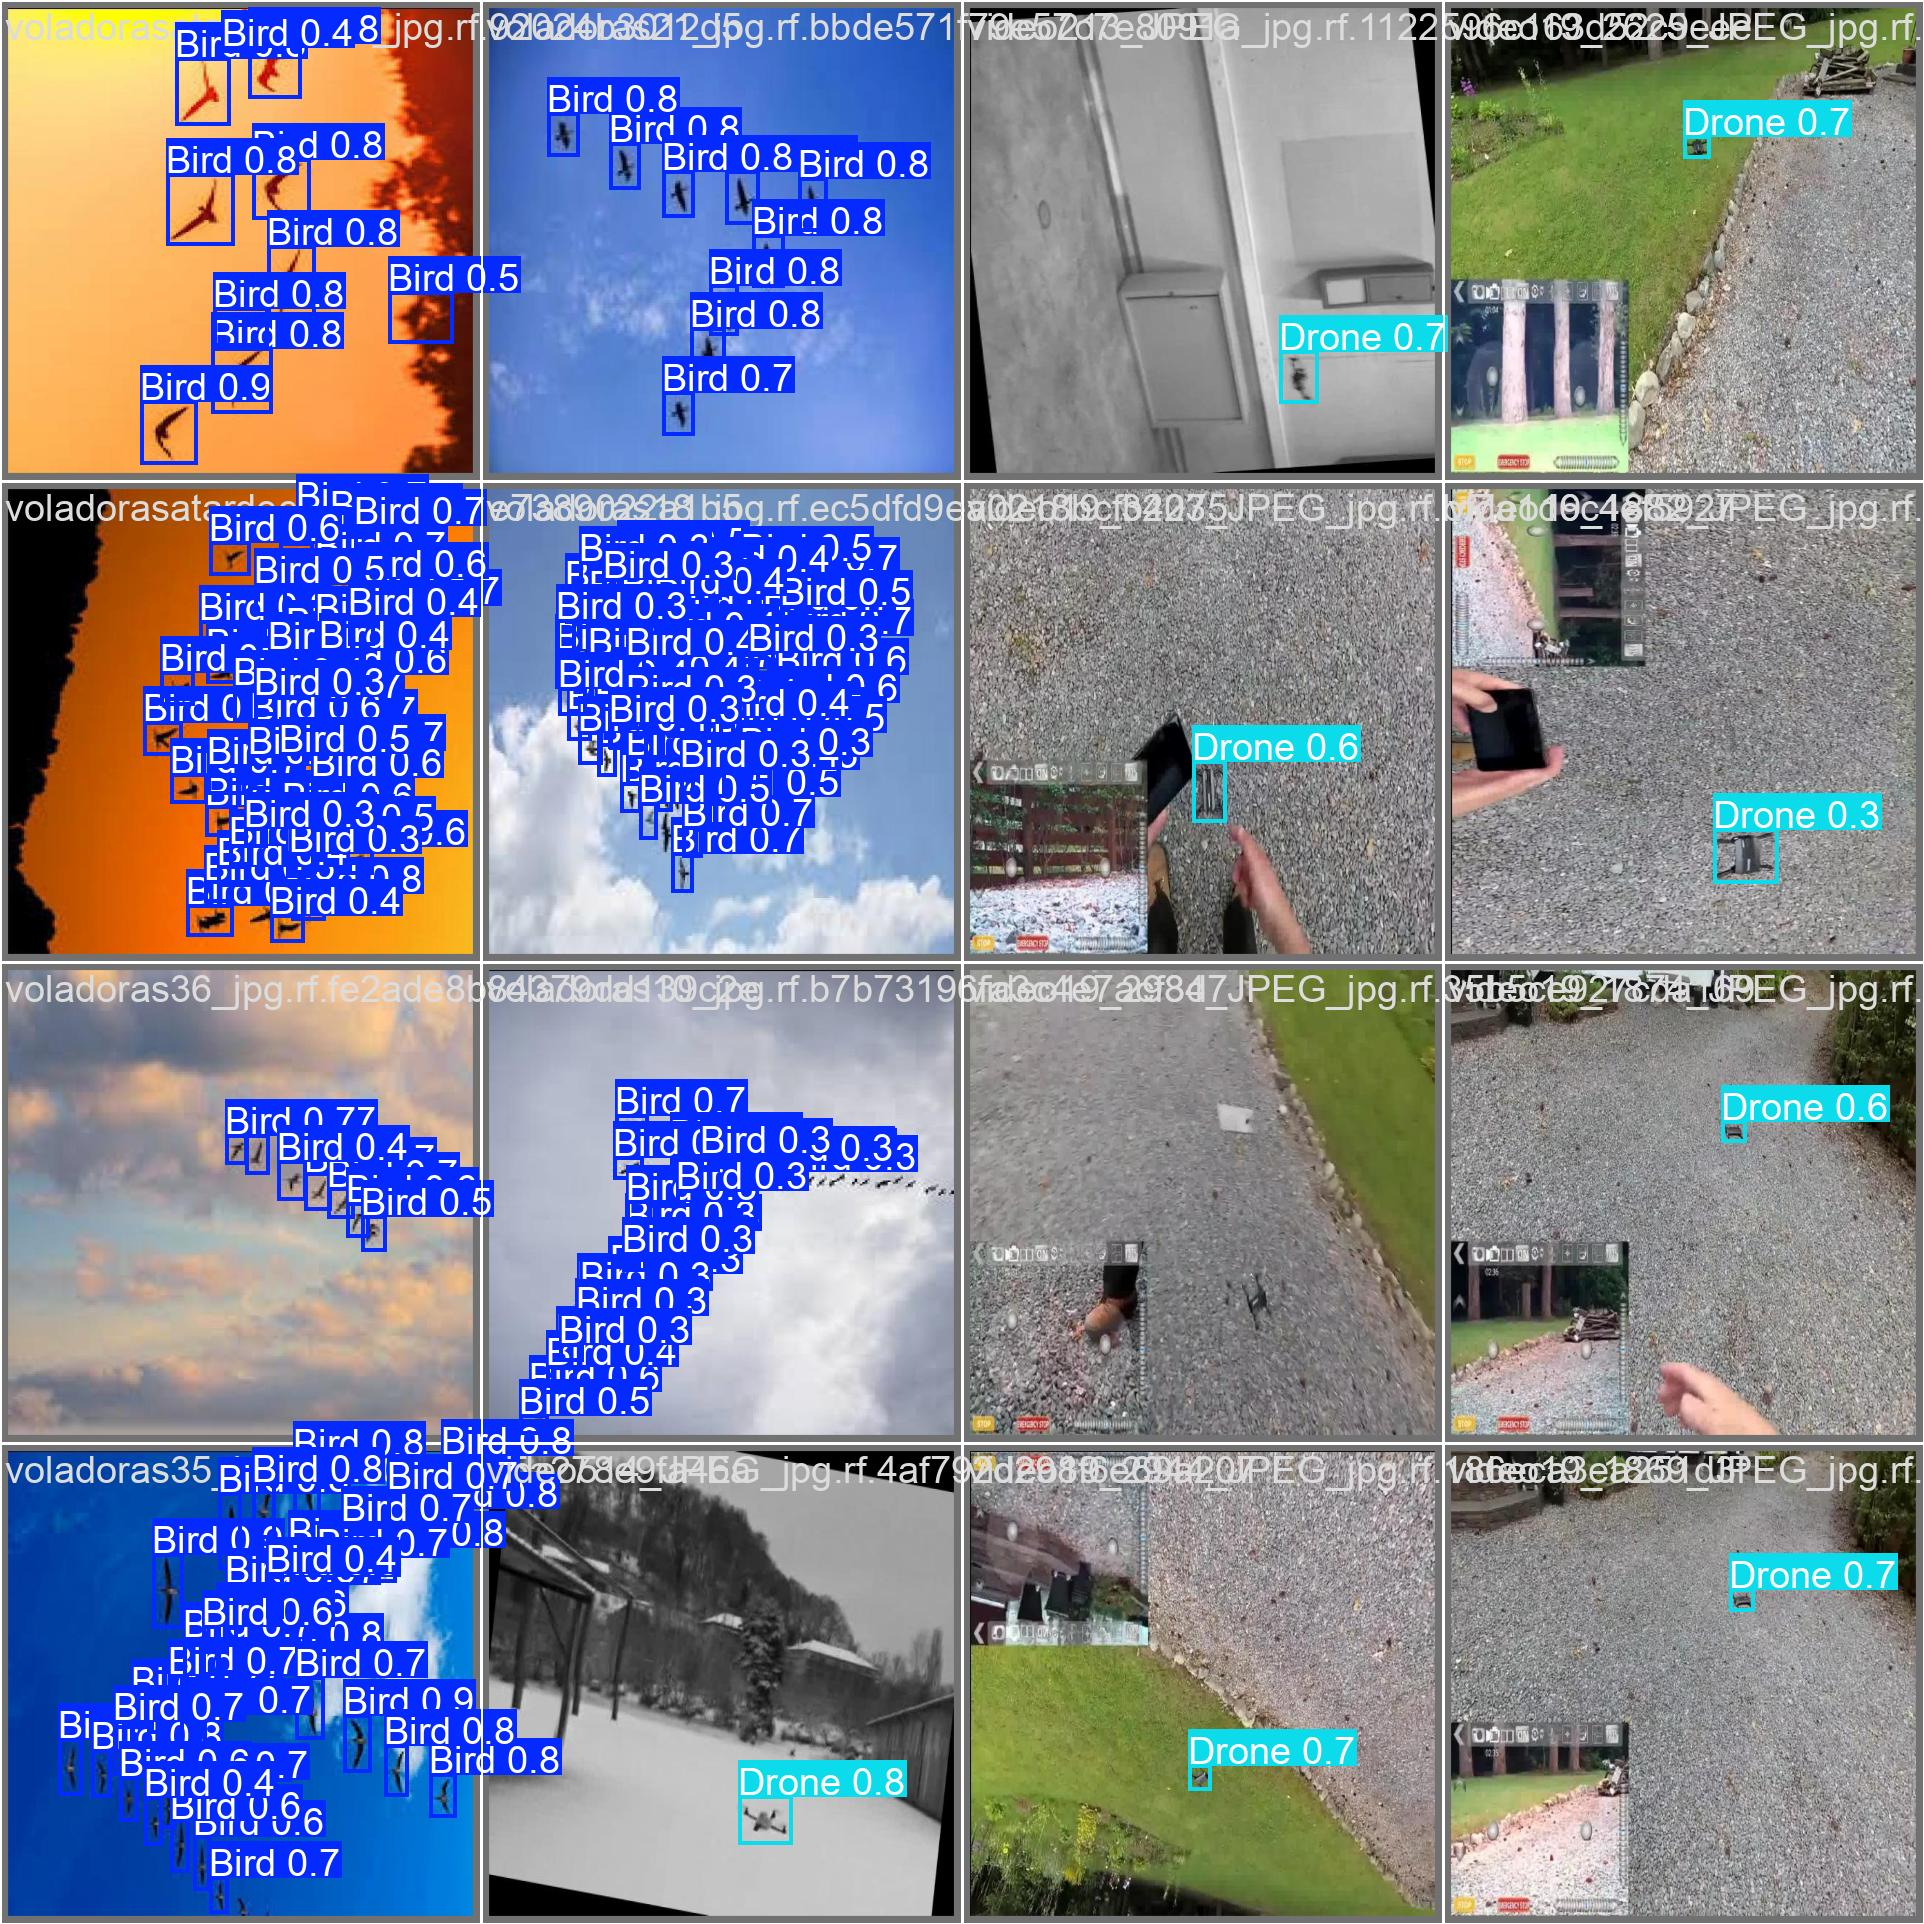
\includegraphics[width=\textwidth]{t2_val_pred.jpg}
\caption{Experiment 2 — Sample validation predictions with bounding boxes}
\label{fig:test2_preds}
\end{figure}

\subsubsection{Discussion}

The two experiments reveal complementary strengths. YOLOv12 Medium achieves
higher mAP50 (91.6\% vs 85.5\%) on the simpler single-class task, benefiting
from the focused training signal. YOLO26s, despite the harder two-class
discrimination task, achieves more balanced precision-recall performance and
demonstrates the effectiveness of YOLO26's STAL and ProgLoss innovations for
handling the visual ambiguity between drones and birds.

The drone-vs-bird confusion matrix (Figure~\ref{fig:test2_confusion}) reveals
the specific failure modes: the model occasionally misclassifies birds as drones
at small apparent sizes, which is the expected failure mode given the visual
similarity at distance. This suggests that incorporating temporal information
(trajectory patterns) alongside spatial features could further improve
discrimination accuracy — a direction for future work.

\subsection{Comparative Summary}

\begin{table}[H]
\centering
\caption{Comparison of Training Experiments}
\begin{tabular}{@{}lllllll@{}}
\toprule
\textbf{Exp.} & \textbf{Model} & \textbf{Classes} & \textbf{mAP50} & \textbf{mAP50-95} & \textbf{Precision} & \textbf{Recall} \\
\midrule
1 & YOLOv12-M & 1 (drone) & 0.916 & 0.493 & 0.988 & 0.778 \\
2 & YOLO26s & 2 (drone+bird) & 0.855 & 0.426 & 0.834 & 0.809 \\
\bottomrule
\end{tabular}
\end{table}

\section{Edge Device Implementation}

\subsection{Camera Acquisition}

The \texttt{CameraSource} module provides unified frame acquisition from USB
cameras (\texttt{/dev/videoN}), RTSP streams, and HTTP MJPEG streams. HTTP
sources use a custom JPEG boundary parser (scanning for \texttt{0xFF 0xD8} /
\texttt{0xFF 0xD9} markers) since \texttt{opencv-python-headless} lacks FFMPEG
support for HTTP URLs. Frames are pushed into a thread-safe queue at the
configured target FPS, with automatic reconnection on disconnection.

\subsection{Inference Pipeline}

The inference pipeline processes frames through the following stages:
(1) frame dequeue from camera buffer;
(2) optional thermal preprocessing (CLAHE + INFERNO colormap);
(3) YOLO inference with ByteTrack tracking via \texttt{model.track()};
(4) payload construction (device ID, timestamp, frame ID, detections);
(5) MQTT publication to \texttt{uav/tracking/\{device\_id\}}.

The \texttt{ModelManager} supports runtime model hot-swapping: inference is
paused, the new model loaded in a background thread, then atomically swapped
without restarting the edge process.

\subsection{MQTT Communication and Security}

All external MQTT communication uses mutual TLS authentication with X.509
certificates generated by the \texttt{certs/gen\_certs.sh} script. The broker
maintains two listeners: port 8883 (TLS, for edge agents) and port 1883 (plain,
internal Docker network only). Tracking payloads use QoS 0 for minimal latency;
status messages use QoS 1 with the retained flag. Last Will and Testament messages
enable automatic offline detection on unexpected disconnection.

\section{Main Device Stack}

The main device runs a Docker Compose stack comprising five services:

\begin{itemize}
  \item \textbf{Mosquitto:} MQTT broker with dual listeners (TLS external / plain internal).
  \item \textbf{Aggregation Service:} FastAPI application subscribing to all UAV
  MQTT topics, maintaining a thread-safe device registry, and exposing REST and
  WebSocket APIs.
  \item \textbf{Control Center:} FastAPI application serving the React frontend
  and proxying API requests to the aggregation service.
  \item \textbf{Signaling Server:} Node.js WebSocket server implementing room-based
  WebRTC signaling (SDP offer/answer and ICE candidate relay).
  \item \textbf{Frontend Builder:} Vite/React build container that compiles the
  TypeScript frontend and copies the output to a shared Docker volume.
\end{itemize}

\section{Frontend Command Center}

The React/TypeScript frontend provides four views:

\begin{itemize}
  \item \textbf{Dashboard:} Tabular device status with inline model switching.
  \item \textbf{Map:} Leaflet.js interactive map with OSM tiles, device markers
  (color-coded by status), detection alert markers, and an unlocated devices panel.
  \item \textbf{Live Feeds:} 2$\times$2 WebRTC video grid with real-time bounding
  box overlays and compact PTZ controls.
  \item \textbf{PTZ Control:} Joystick-based pan/tilt control with zoom buttons
  and absolute position inputs.
\end{itemize}

\begin{figure}[H]
\centering
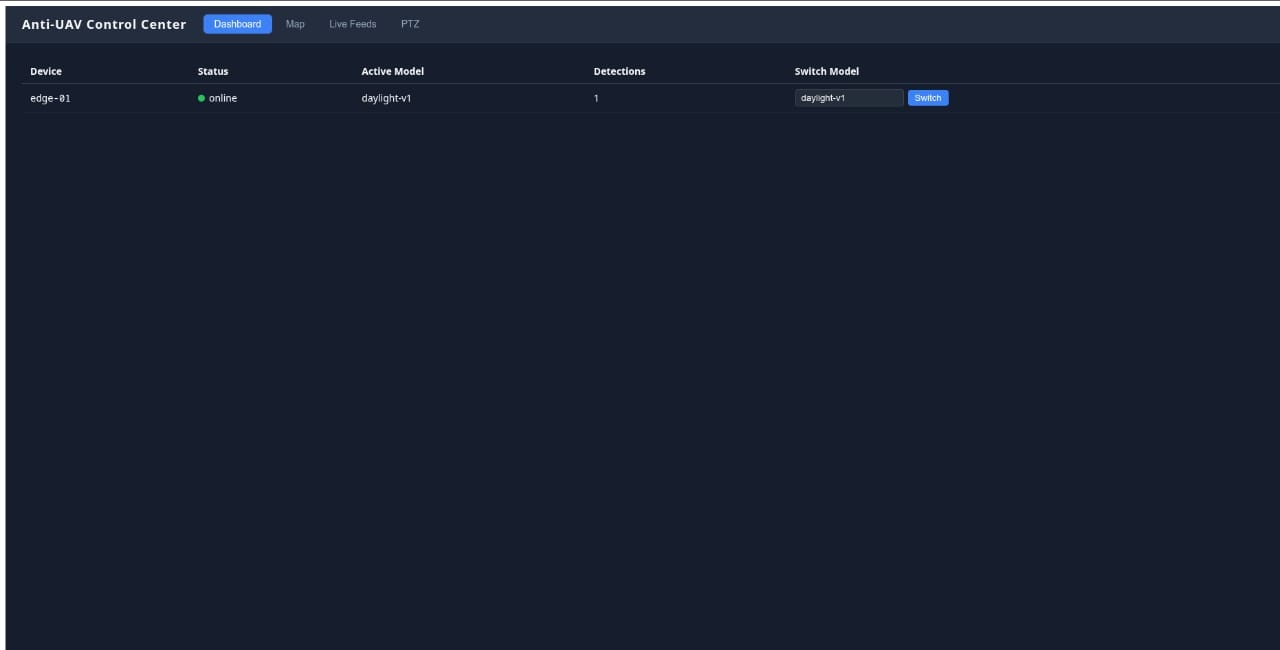
\includegraphics[width=\textwidth]{Control_Center_Overview.jpg}
\caption{Anti-UAV Control Center — main dashboard view}
\label{fig:cc_overview}
\end{figure}

\begin{figure}[H]
\centering
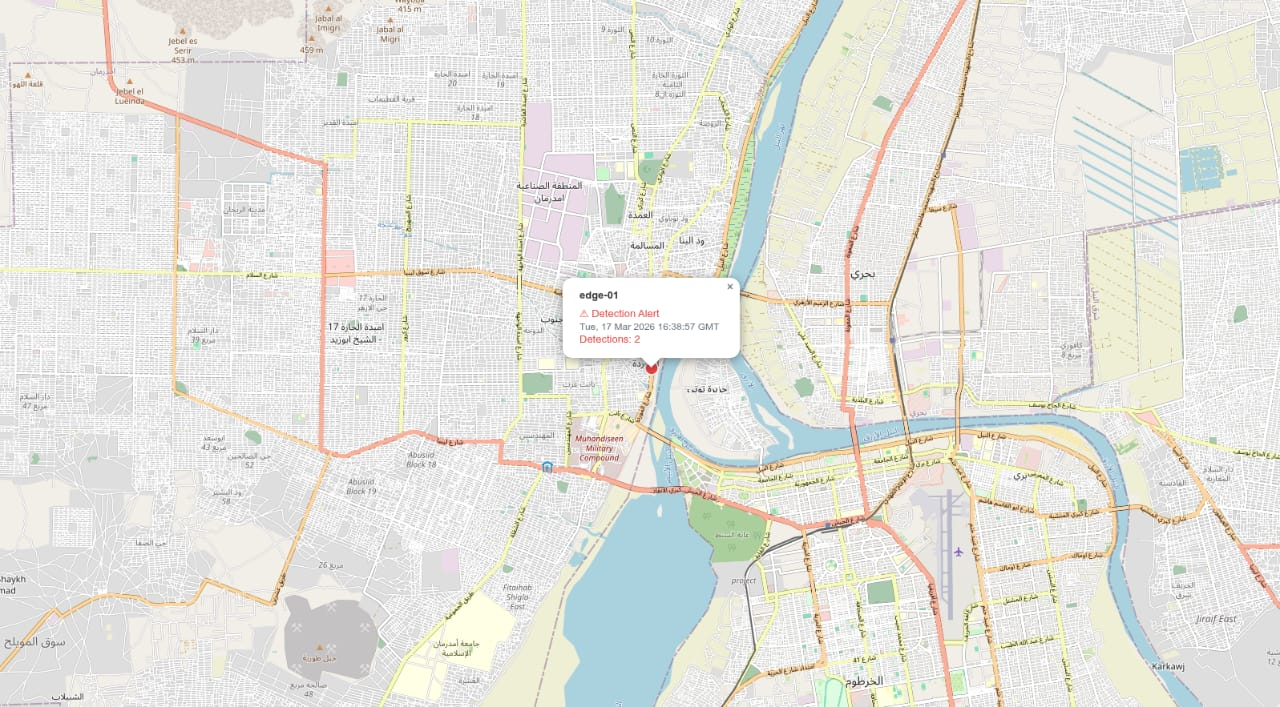
\includegraphics[width=\textwidth]{Control_Center_Map.jpg}
\caption{Map view — geospatial device tracking with OpenStreetMap tiles}
\label{fig:cc_map}
\end{figure}

\begin{figure}[H]
\centering
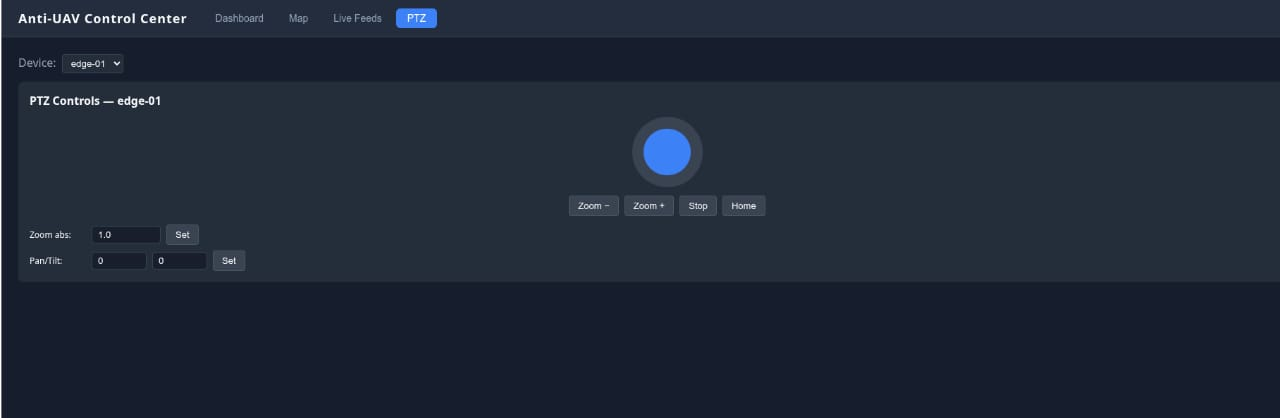
\includegraphics[width=0.7\textwidth]{Control_Center_PTZ_Controls.jpg}
\caption{PTZ control panel — joystick pan/tilt and zoom controls}
\label{fig:cc_ptz}
\end{figure}

\section{Launcher GUIs}

Two Tkinter-based GUI launchers simplify system operation:
\texttt{launcher\_main.py} configures and starts the Docker stack on the main
device; \texttt{launcher\_edge.py} configures camera, MQTT, TLS certificates,
and model paths on the edge device, then launches the inference process.

\section{Testing}

The system includes 138 passing unit and integration tests covering all components,
implemented with \texttt{pytest}, \texttt{pytest-asyncio}, and \texttt{hypothesis}
for property-based testing.

% ══════════════════════════════════════════════════════════════════════════════
% BIBLIOGRAPHY
% ══════════════════════════════════════════════════════════════════════════════
\bibliographystyle{IEEEtran}
\begin{thebibliography}{99}

\bibitem{zhao2019object}
Z.~Zhao, P.~Zheng, S.~Xu, and X.~Wu,
``Object Detection with Deep Learning: A Review,''
\textit{IEEE Trans. Neural Netw. Learn. Syst.}, vol.~30, no.~11, pp.~3212--3232, 2019.

\bibitem{lecun2015deep}
Y.~LeCun, Y.~Bengio, and G.~Hinton,
``Deep Learning,''
\textit{Nature}, vol.~521, pp.~436--444, 2015.

\bibitem{redmon2016yolo}
J.~Redmon, S.~Divvala, R.~Girshick, and A.~Farhadi,
``You Only Look Once: Unified, Real-Time Object Detection,''
in \textit{Proc. IEEE CVPR}, 2016, pp.~779--788.

\bibitem{girshick2014rcnn}
R.~Girshick, J.~Donahue, T.~Darrell, and J.~Malik,
``Rich Feature Hierarchies for Accurate Object Detection and Semantic Segmentation,''
in \textit{Proc. IEEE CVPR}, 2014, pp.~580--587.

\bibitem{ren2015fasterrcnn}
S.~Ren, K.~He, R.~Girshick, and J.~Sun,
``Faster R-CNN: Towards Real-Time Object Detection with Region Proposal Networks,''
in \textit{Adv. Neural Inf. Process. Syst.}, vol.~28, 2015.

\bibitem{sapkota2025yolo26}
R.~Sapkota and M.~Karkee,
``YOLO26: Key Architectural Enhancements and Performance Benchmarking for Real-Time Object Detection,''
\textit{arXiv:2509.25164v4}, 2026.

\bibitem{reis2023yolov8flying}
D.~Reis, J.~Hong, J.~Kupec, and A.~Daoudi,
``Real-Time Flying Object Detection with YOLOv8,''
\textit{arXiv:2305.09972v2}, 2024.

\bibitem{zhang2022bytetrack}
Y.~Zhang \textit{et al.},
``ByteTrack: Multi-Object Tracking by Associating Every Detection Box,''
in \textit{Proc. ECCV}, 2022, pp.~1--21.

\bibitem{delleji2024thermal}
T.~Delleji, F.~Slimeni, and A.~Siala,
``Good Data Beats More Data: Building a Thermal Air-Image Dataset for Ground-to-Air Surveillance,''
in \textit{Transfer Learning -- Unlocking the Power of Pretrained Models}, IntechOpen, 2024.

\bibitem{shi2016edge}
W.~Shi, J.~Cao, Q.~Zhang, Y.~Li, and L.~Xu,
``Edge Computing: Vision and Challenges,''
\textit{IEEE Internet Things J.}, vol.~3, no.~5, pp.~637--646, 2016.

\bibitem{stacker2021edge}
M.~Stacker \textit{et al.},
``Deployment of Deep Neural Networks for Object Detection on Edge Devices,''
in \textit{Proc. IEEE/CVF ICCV Workshops}, 2021.

\bibitem{mqtt5spec}
OASIS Standard,
``MQTT Version 5.0,'' 2019.
[Online]. Available: \url{https://docs.oasis-open.org/mqtt/mqtt/v5.0/mqtt-v5.0.html}

\bibitem{webrtcspec}
W3C and IETF,
``WebRTC 1.0: Real-Time Communication Between Browsers,''
W3C Recommendation, 2021.
[Online]. Available: \url{https://www.w3.org/TR/webrtc/}

\bibitem{merkel2014docker}
D.~Merkel,
``Docker: Lightweight Linux Containers for Consistent Development and Deployment,''
\textit{Linux Journal}, vol.~2014, no.~239, 2014.

\end{thebibliography}

\end{document}
